\documentclass[UTF8,a4paper,12pt]{ctexart}

% 页面设置
\usepackage{geometry}
\geometry{
  left=2.5cm,
  right=2.5cm,
  top=2.5cm,
  bottom=2.5cm
}

% 数学公式
\usepackage{amsmath,amssymb}

% 插入图片
\usepackage{graphicx}
\usepackage{placeins}

% 表格
\usepackage{booktabs}
\usepackage{tabularx}

% 超链接
\usepackage[colorlinks=true,linkcolor=blue,citecolor=blue]{hyperref}

\title{\textbf{基于某模型的某问题研究}}

\begin{document}

% 第一页
\maketitle

\begin{abstract}
本文针对某问题建立数学模型。首先……；其次……；
最后通过数值实验验证模型的有效性。

\textbf{关键词：} 数学建模；优化模型；数值分析
\end{abstract}

% 正文开始

\newpage

\section{问题背景与重述}
\subsection{问题背景}
无线电干扰源的定位与清除是无线电频谱管理的重要任务。通过固定监测站、移动监测车或无人机开展初步监测与区域排查后，通常能够确定干扰源的大致分布范围。然而，受环境遮挡和干扰源功率等因素影响，精准定位仍需技术人员携带测向设备进入目标区域，依据多次检测结果逐步缩小搜索范围。为缩短干扰持续时间，并减少人员在危险环境中的作业风险，有必要研究搭载于机器狗的自动定位与清除方法。

测向机通过接收信号获得干扰源相对于检测点的方位信息，但受测量误差影响，单次示向度只能限定目标所在的一个角度范围。不同位置的观测可以进一步收紧定位区域，其效果与检测点的空间分布有关。此外，测向机的有效接收距离有限；对于具有特定辐射方向的干扰源，即使距离较近，也可能无法接收到信号。因此，检测结果既受到目标位置的影响，也与接收范围和辐射方向有关。

机器狗需要在移动、切换频道和停驻检测之间作出安排，并在接近干扰源后完成光学精确定位与清除。这些操作均消耗时间，单纯追求更小的定位区域未必能够缩短整个任务的耗时。因而，需要将\textbf{定位精度与搜索清除效率}结合起来，在确保所有干扰源被清除的前提下，合理选择检测位置并规划后续行动。
\subsection{问题重述}
题目已将干扰源的分布范围限定为半径为 $1800\,\mathrm m$ 的圆域，并给出了测向误差、有效接收距离及各项操作的时间与距离约束。根据所提供的信息，需要建立数学模型解决以下问题。

\textbf{问题一：}已知多个检测点的坐标及同一干扰源在各点的示向度，设计交会定位区域的构造与直径计算方法，并判断是否存在以该区域直径为直径、能够覆盖整个定位区域的圆盘。

\textbf{问题二：}已知某全向干扰源在第一个检测点处的示向度，明确较好定位效果的评价依据，制定第二个检测点的选择策略，并给出相应的候选区域。

\textbf{问题三：}目标区域内有 $10$--$16$ 个全向干扰源，具体数量未知。机器狗从原点出发，初始检测频道为 $1$，要求在\textbf{确保全部清除}的前提下尽量缩短任务总时间。设计自动搜索、定位与清除算法，通过模拟器演练统计清除比例和平均定位清除时间，并完成三次正式测试，报告结果及保存相应日志。

\textbf{问题四：}将目标扩展为全向与定向干扰源混合的情形，总数仍为 $10$--$16$ 个，定向源的数量和辐射方向均未知。在其余条件与问题三相同的情况下，制定适用的检测与清除策略，检验算法的有效性，并按要求完成三次正式测试及结果记录。


\section{问题分析}
\subsection{问题一}

考虑示向度误差后，每次检测可将干扰源限制在一个楔形区域内，全部楔形的交集即为本问的定位区域。
本问需解决三个相关的问题：如何完整构造该区域，如何求出连续区域内的最大点间距，
以及是否存在直径与该最大距离相同的圆盘覆盖整个区域。
为此，将测向约束写成半平面不等式，利用凸多边形的顶点表示将直径计算化为有限点对比较，
再由直径端点确定可能的覆盖圆心，建立覆盖判据，最后用 $10$ 个检测点的随机算例检验计算流程。


\subsection{问题二}
第一次检测只能确定干扰源的大致方向，第二个检测点的位置会影响两次检测后的定位范围。
选点既需改善测向交会的几何关系，也需考虑接收范围对反馈的影响。
因此，以最小覆盖圆半径衡量定位效果，根据首次观测预测各测点的全部可能反馈，
比较反馈后的期望覆盖半径，给出推荐测点及近优候选区域，并通过两组初始条件和简单策略对照解释选点结果。
\subsection{问题三}
···
\subsection{问题四}
定向源在发射方向的背面不产生信号，因此，问题三中利用单次无信号排除邻近区域的方法不再适用。
本问先根据半平面辐射特征，建立多个无信号测点的联合排除条件，
再布置能够搜索整个目标圆域的检测点，避免遗漏尚未发现的源。
对于已发现的源，需要同时考虑其位置、接收半径和发射方向，判断哪些情形能够解释已有观测。
在此基础上，沿用问题三的时间评价安排后续检测与清除，并通过相同地图上的对照实验检验效果。


\section{模型假设}
\label{sec:assumptions}

在题设场景下，我们作出如下假设与计算约定。
\begin{enumerate}
  \item \textbf{任务期间外部环境保持稳定。}干扰源位置不随时间变化，环境对信号接收的影响由题设的有效接收范围和测角误差描述，不另行考虑突发遮挡、设备故障等因素。
  \item \textbf{检测点坐标可准确获得。}忽略机器狗自身定位误差及运动控制误差，忽略地形高度变化、加减速和转向等造成的额外耗时。
  \item \textbf{采用均匀测角误差模型。}对同一干扰源，假设示向度相对真实方位角的误差在 $[-1^\circ,1^\circ]$ 内均匀分布，并认为不同检测位置的误差相互独立。
  \item \textbf{采用面积均匀的位置先验。}在尚未获得某干扰源的观测信息时，假设其出现在目标圆域内等面积区域的概率相同；获得检测反馈后，再更新其位置分布。
\end{enumerate}

\section{符号说明}
全文沿用表~\ref{tab:symbol} 的符号。下标 $i=1,\ldots,n$ 表示检测点，
$j,k=1,\ldots,m$ 表示多边形顶点；坐标分量用下标 $x,y$ 区分。
角度以正东方向为零点、逆时针为正，计算时使用弧度。
\begin{table}[htbp]
  \centering
  \caption{主要符号及约定}
  \label{tab:symbol}
  \label{tab:q1-symbols}
  \begin{tabularx}{\linewidth}{lX}
    \toprule
    符号 & 含义 \\
    \midrule
    $n,\,m$ & 检测点数、定位多边形的顶点数 \\
    $\boldsymbol p_i=(p_{i,x},p_{i,y})^{\mathsf T}$ & 第 $i$ 个检测点的平面坐标（$\mathrm m$） \\
    $\theta_i,\,\varepsilon$ & 第 $i$ 个检测点的示向度、误差上界，$\varepsilon=\pi/180$ \\
    $\boldsymbol n_i^-,\,\boldsymbol n_i^+$ & 第 $i$ 个楔形的两条边界的向内单位法向量；上标 $-,+$ 对应 $\theta_i-\varepsilon,\theta_i+\varepsilon$ \\
    $W_i,\,P$ & 第 $i$ 个楔形区域、全部楔形的交集 \\
    $\boldsymbol x,\,\boldsymbol s$ & 待判断的位置、模拟数据中的真实源位置（$\mathrm m$） \\
    $\boldsymbol v_j$ & 按逆时针排序的第 $j$ 个多边形顶点（$\mathrm m$） \\
    $D;\ \boldsymbol a,\boldsymbol b$ & 区域直径及取得直径的一对顶点（$\mathrm m$） \\
    $\boldsymbol c_D$ & 以 $\boldsymbol a\boldsymbol b$ 为直径的圆心（$\mathrm m$） \\
    $R_*,\,\boldsymbol c_*$ & 最小覆盖圆的半径和圆心（$\mathrm m$） \\
    \bottomrule
  \end{tabularx}
\end{table}

\section{模型建立与求解}
\subsection{问题一模型建立}
\label{sec:q1}
% 按整合修改意见修订问题一；单位与符号统一、图像素材核对仍留待后续。

\subsubsection{定位区域}
\label{sec:q1-wedge}




本问的定位多边形指全部示向约束形成的楔形交集，不叠加距离或圆形活动范围的裁剪；
若加入这些约束，边界可能含有圆弧，需另行处理。
示向度误差为 $\pm1^\circ$，因此干扰源应在 $\theta_i-\varepsilon$ 与
$\theta_i+\varepsilon$ 两条射线夹成的楔形内。直接比较角度需要处理跨越 $0^\circ$ 的情况，
这里改用\textbf{法向量内积判断点位于边界的哪一侧}。
将下侧边界的方向向量逆时针旋转 $90^\circ$，上侧边界的方向向量顺时针旋转 $90^\circ$，得到
\[
  \begin{aligned}
    \boldsymbol n_i^-&=\bigl(-\sin(\theta_i-\varepsilon),\ \cos(\theta_i-\varepsilon)\bigr)^{\mathsf T},\\
    \boldsymbol n_i^+&=\bigl(\sin(\theta_i+\varepsilon),\ -\cos(\theta_i+\varepsilon)\bigr)^{\mathsf T}.
  \end{aligned}
\]
这两个单位法向量分别朝向各自边界包含楔形的那一侧，于是
\begin{equation}
  W_i=\left\{\boldsymbol x\in\mathbb R^2:
  (\boldsymbol n_i^-)^{\mathsf T}(\boldsymbol x-\boldsymbol p_i)\geq0,\quad
  (\boldsymbol n_i^+)^{\mathsf T}(\boldsymbol x-\boldsymbol p_i)\geq0\right\}.
  \label{eq:q1-wedge}
\end{equation}


式~\eqref{eq:q1-wedge} 中，$\boldsymbol x-\boldsymbol p_i$ 是从检测点指向待判断位置的向量，
它与单位法向量的内积，就是沿该法向量的投影，也就是到边界直线的有向距离。
\textbf{内积为正时，点在朝向楔形内部的一侧；为零时在边界上；为负时在外侧。}
两项必须同时非负，才能说明该点位于两条射线之间。
例如，沿示向方向前进距离 $t>0$，两项内积都为 $t\sin\varepsilon>0$；
若反向移动，则两项均为负。因此，该判据也排除了检测点后方的区域。




将每次检测的两个约束合并，可得
\begin{equation}
  P=\bigcap_{i=1}^{n}W_i=\{\boldsymbol x:H\boldsymbol x\leq\boldsymbol g\}.
  \label{eq:q1-intersection}
\end{equation}
矩阵 $H$ 的第 $2i-1,2i$ 行分别为 $-(\boldsymbol n_i^-)^{\mathsf T}$、
$-(\boldsymbol n_i^+)^{\mathsf T}$，$\boldsymbol g$ 的对应分量为这两行与 $\boldsymbol p_i$ 的乘积。
对任意 $\boldsymbol x,\boldsymbol y\in P$ 及 $\lambda\in[0,1]$，有
\[
  H\bigl(\lambda\boldsymbol x+(1-\lambda)\boldsymbol y\bigr)
  \leq\lambda\boldsymbol g+(1-\lambda)\boldsymbol g=\boldsymbol g.
\]
因此两点间的整条线段仍在 $P$ 内，故 $P$ 为凸集，这也是交集保凸性的直接体现。
下文先讨论 $P$ 非空、有界且内部非空的情形，此时它是凸多边形。
由有界多面体的顶点表示定理\cite{boyd2004convex}，
$P=\operatorname{conv}(V)$，其中 $V=\{\boldsymbol v_1,\ldots,\boldsymbol v_m\}$ 为全部顶点集合，
$\operatorname{conv}(V)$ 表示顶点所有凸组合构成的集合。


\begin{figure}[htbp]
  \centering
  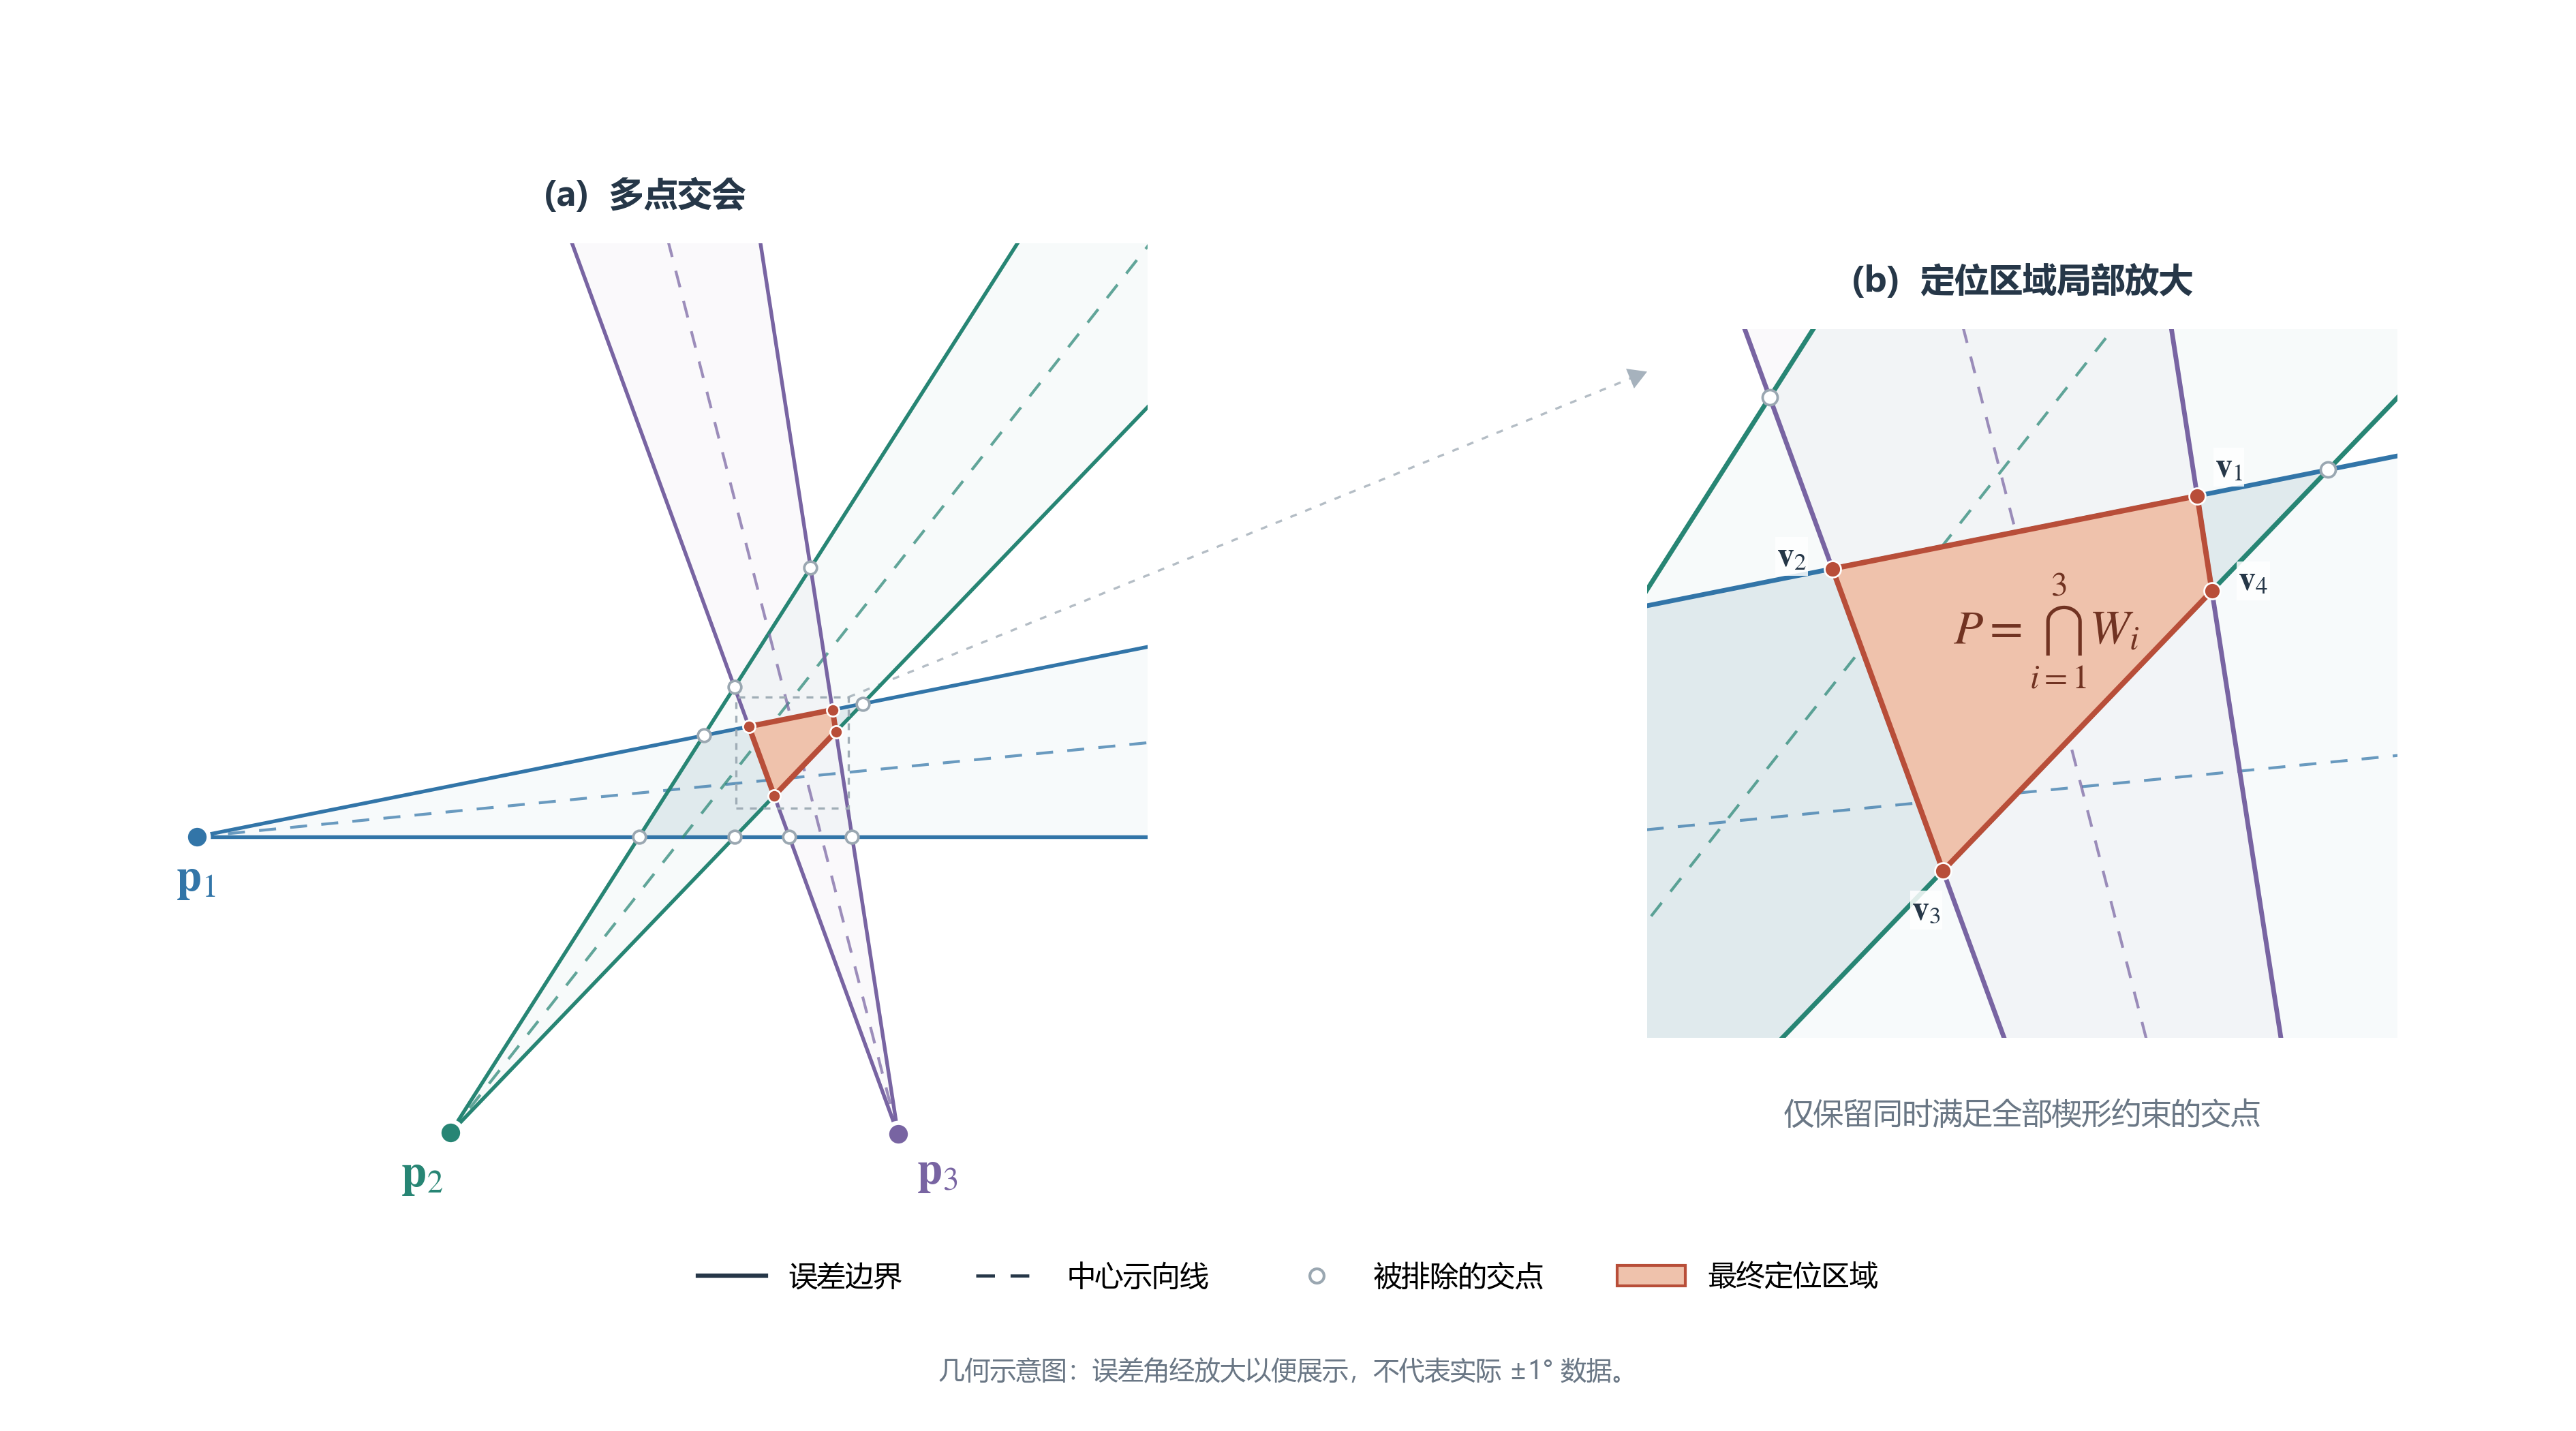
\includegraphics[width=0.94\linewidth]{data/q1_wedge_intersection/q1_wedge_intersection.png}
  \caption{楔形交会与定位区域（误差角放大示意）}
  \label{fig:q1-wedges}
\end{figure}




\label{sec:q1-filter}
\label{sec:q1-polygon}
求取多边形时，最直接的办法是\textbf{枚举边界交点}。
将 $2n$ 条边界射线所在的直线作为候选边界，仅对不平行的直线求交，
再用式~\eqref{eq:q1-intersection} 的全部约束筛选；平行或重合直线不作为唯一交点的来源。
保留点去重后求凸包，得到按逆时针排列的顶点，无须额外判断射线参数。
记保留点集为 $S_{\mathrm f}$。每个多边形顶点至少位于两条不平行的活跃边界上
（即对应不等式在该点取等号），否则该点可沿边界方向向两侧移动而仍保持可行，不能成为顶点。
因此枚举不会遗漏顶点，且筛选保证 $V\subseteq S_{\mathrm f}\subseteq P$，从而
\[
  P=\operatorname{conv}(V)\subseteq\operatorname{conv}(S_{\mathrm f})\subseteq P.
\]
这证明所得凸包恰好是完整定位区域。候选交点为 $O(n^2)$ 个，每点检查 $2n$ 个约束，
连同去重和凸包计算，区域构造复杂度为 $O(n^3)$。

另一种办法是直接求\textbf{半平面交}。先将边界统一为可行半平面位于左侧的有向直线，
按方向角排序，同向平行边界仅保留较严格者；再用双端队列维护有效边界。
加入新约束时，删除队首或队尾使相邻交点落在新半平面外侧的边界，最后检查首尾闭合。
排序耗时 $O(n\log n)$，每条边界至多入队、出队一次，故区域构造复杂度为 $O(n\log n)$。
交点枚举便于逐项检查约束，半平面交降低构造阶段的渐近复杂度；两者基于同一模型，结果比较用于核对实现。

算法还需识别区域状态：空集表示约束不相容，非空无界区域没有有限直径；
退化为点或有界线段时，直径分别为零或线段长度。
不能仅凭没有找到交点判断为空，也不能以人为边框将无界区域当成有界多边形。


\subsubsection{区域直径}
\label{sec:q1-diameter}




区域直径描述仍与观测相容的任意两个位置之间的最大距离。
由于 $P$ 是闭且有界的非空多边形，该最大值能够取得。

\noindent\textbf{命题1（顶点直径）}\quad 定位多边形的直径可由一对顶点取得，即
\begin{equation}
  D=\max_{\boldsymbol x,\boldsymbol y\in P}\|\boldsymbol x-\boldsymbol y\|_2
   =\max_{1\leq j,k\leq m}\|\boldsymbol v_j-\boldsymbol v_k\|_2.
  \label{eq:q1-vertex-diameter}
\end{equation}
\noindent\textbf{证明：}由 $P=\operatorname{conv}(V)$，任意 $\boldsymbol x,\boldsymbol y\in P$ 均可写成顶点的凸组合
$\boldsymbol x=\sum_j\alpha_j\boldsymbol v_j$、$\boldsymbol y=\sum_k\beta_k\boldsymbol v_k$，
其中权重非负且各自的和为 $1$。由三角不等式，
\[
  \|\boldsymbol x-\boldsymbol y\|_2
  =\left\|\sum_{j,k}\alpha_j\beta_k(\boldsymbol v_j-\boldsymbol v_k)\right\|_2
  \leq\sum_{j,k}\alpha_j\beta_k\|\boldsymbol v_j-\boldsymbol v_k\|_2
  \leq\max_{j,k}\|\boldsymbol v_j-\boldsymbol v_k\|_2.
\]
又因顶点本身属于 $P$，等号可以由一对最远顶点取得。
因此，无须对区域内部进行空间采样，枚举顶点对即可在 $O(m^2)$ 时间内求出 $D$，
并记录对应端点 $\boldsymbol a,\boldsymbol b$。该化简消除了空间网格近似，但计算仍受浮点精度影响。


\subsubsection{圆的覆盖}
\label{sec:q1-cover-counterexample}
\label{sec:q1-cover-condition}




下文所称覆盖圆均指包含内部及边界的闭圆盘，记
$B(\boldsymbol c,r)=\{\boldsymbol x:\|\boldsymbol x-\boldsymbol c\|_2\leq r\}$。
取直径端点 $\boldsymbol a,\boldsymbol b$，记其中点为 $\boldsymbol c_D=(\boldsymbol a+\boldsymbol b)/2$。
若半径为 $D/2$、圆心为 $\boldsymbol o$ 的圆盘能覆盖 $P$，则必包含这两个端点，故
\[
  D=\|\boldsymbol a-\boldsymbol b\|_2
  \leq\|\boldsymbol a-\boldsymbol o\|_2+\|\boldsymbol o-\boldsymbol b\|_2\leq D.
\]
两处均须取等，因而 $\boldsymbol o$ 在线段 $\boldsymbol a\boldsymbol b$ 上，
且到两端点的距离均为 $D/2$，即 $\boldsymbol o=\boldsymbol c_D$。
所以满足要求的覆盖圆若存在，其圆心只能是该中点。

然而，中点圆不一定覆盖整个区域。例如，边长为 $D>0$ 的等边三角形，
任取一条边，其对顶点到该边中点的距离为 $\sqrt{3}D/2>D/2$。
结合圆心唯一性可知，不存在半径为 $D/2$ 的圆盘覆盖该三角形。
图~\ref{fig:q1-cover-cases} 给出了三个检测点的楔形交形成三角形时，不能覆盖与可以覆盖的两种情形，
各楔形张角均为 $2^\circ$。


\begin{figure}[htbp]
  \centering
  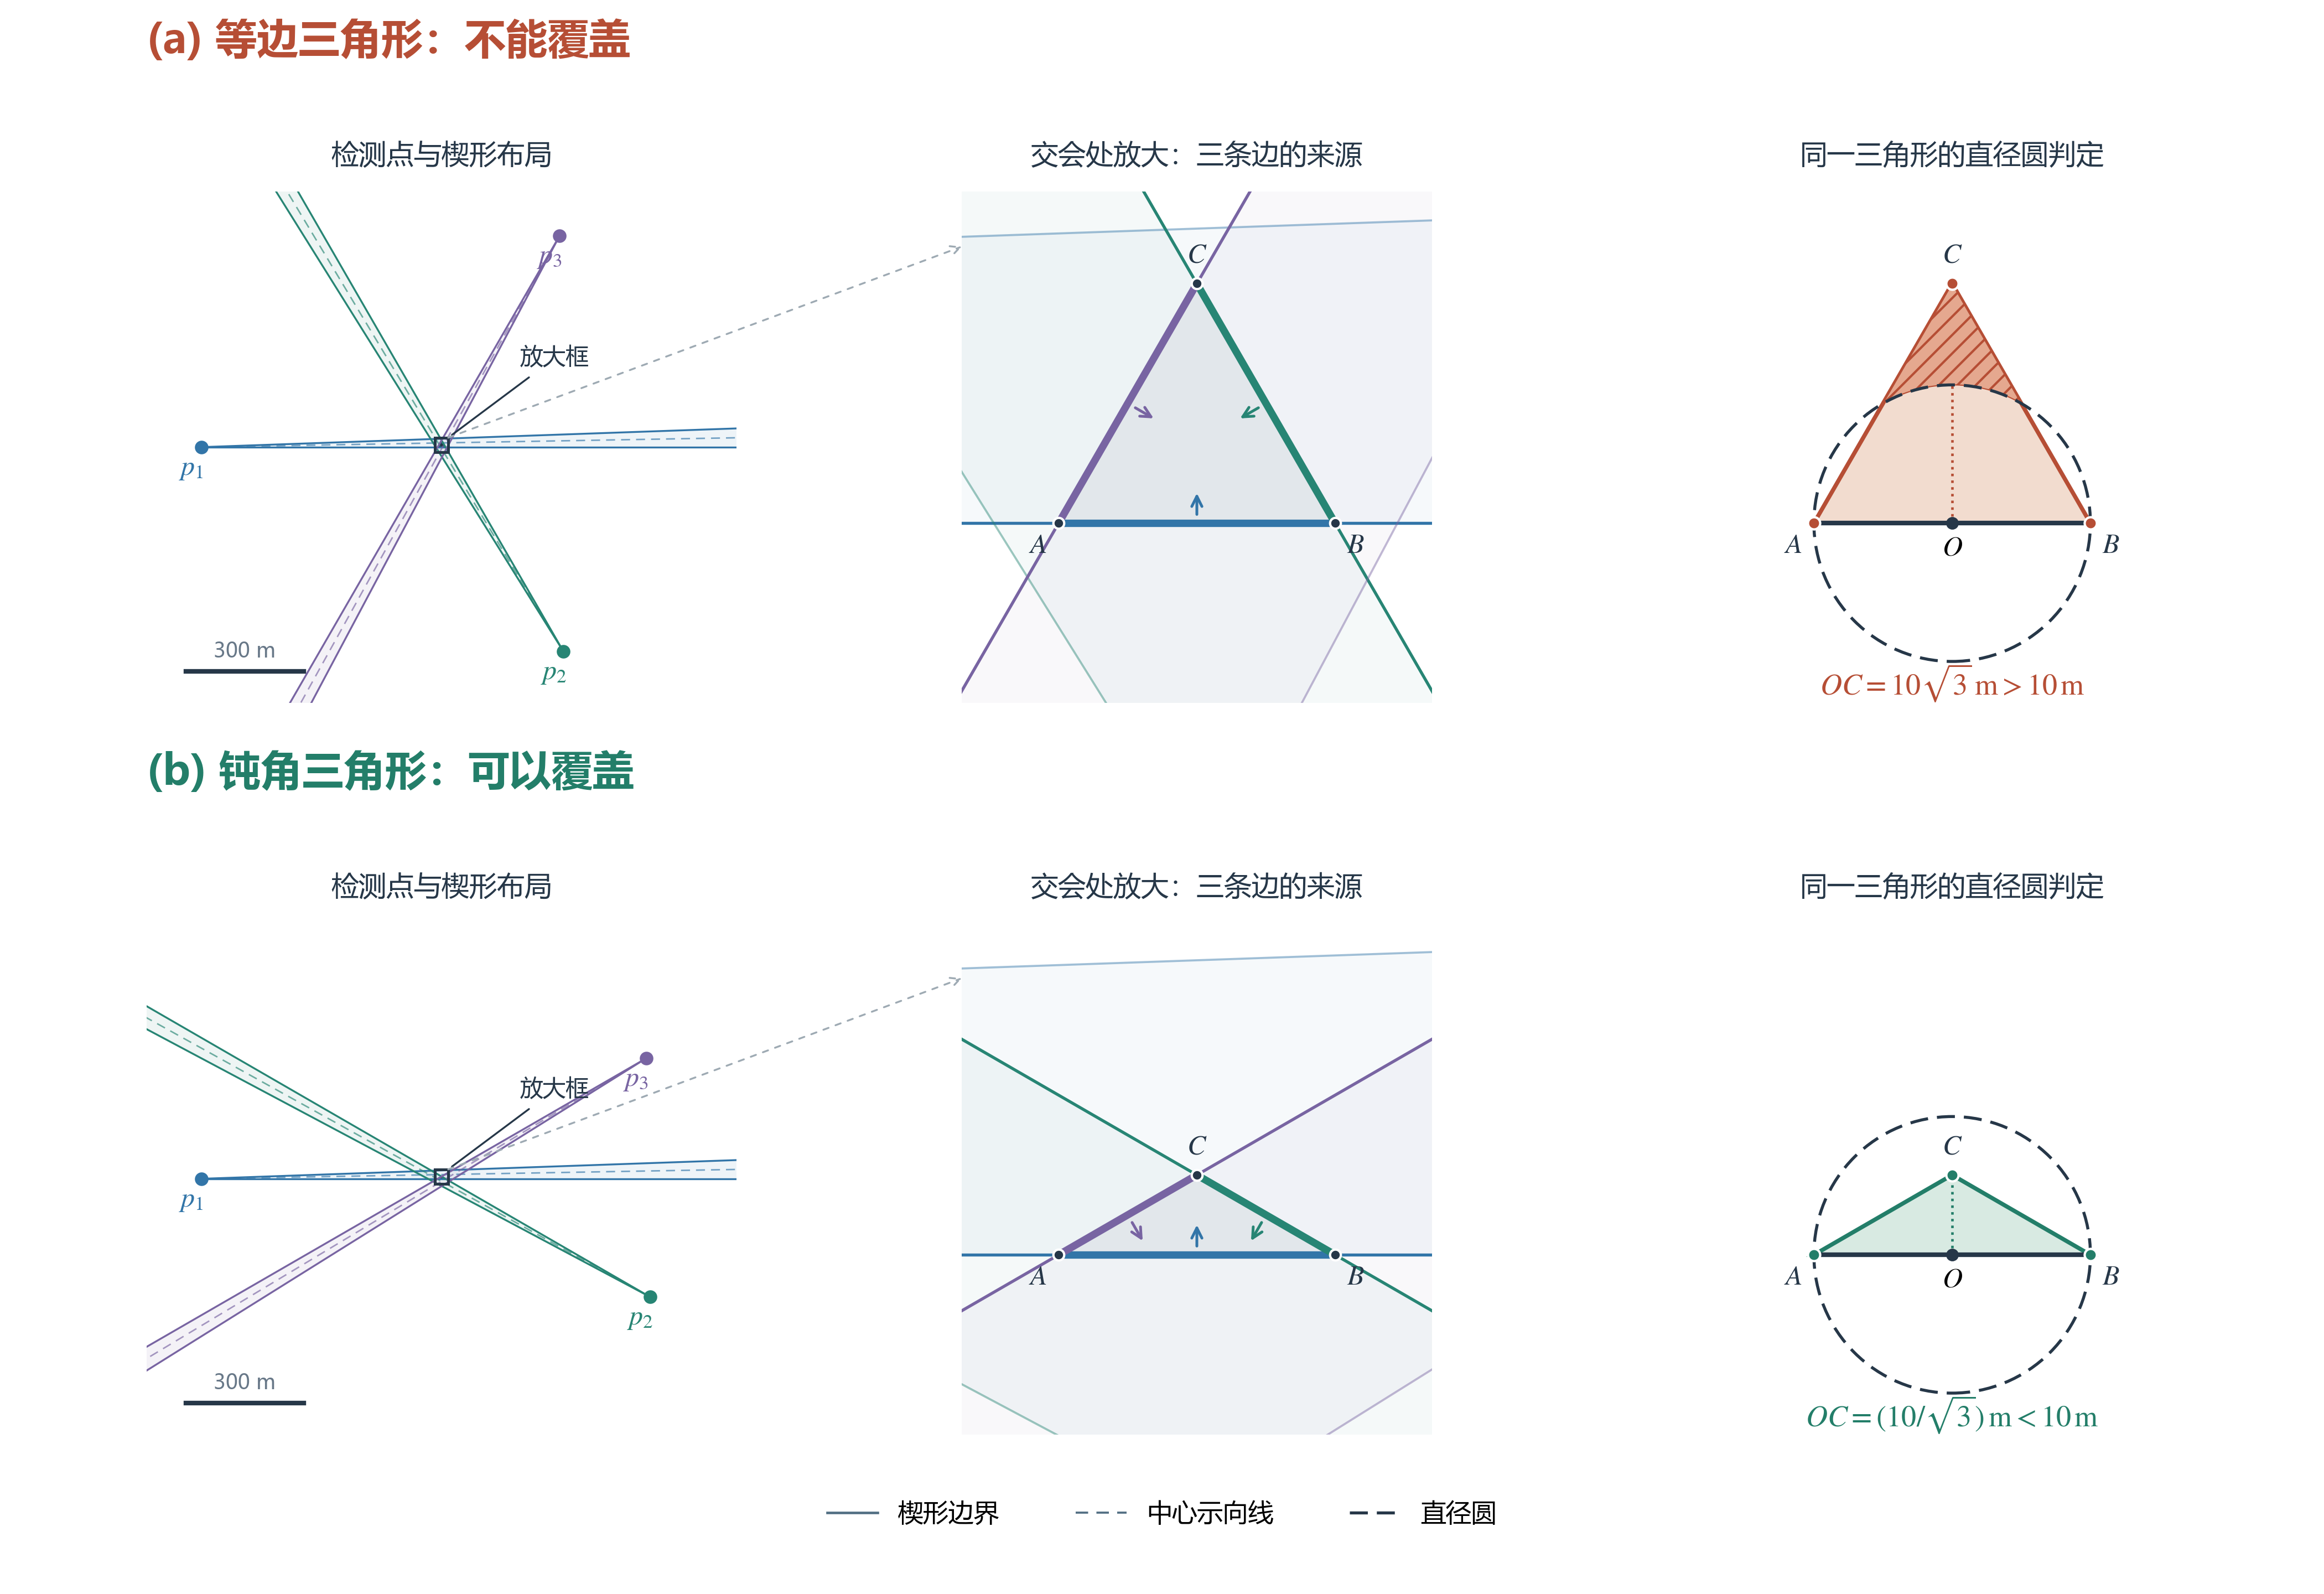
\includegraphics[width=0.84\linewidth]{data/q1_cover_cases/q1_cover_cases.png}
  \caption{直径圆不能覆盖与可以覆盖的情形}
  \label{fig:q1-cover-cases}
\end{figure}




\noindent\textbf{命题2（直径圆覆盖判据）}\quad 对定位多边形 $P$，有
\begin{equation}
  \exists\,\boldsymbol o:\ P\subseteq B(\boldsymbol o,D/2)
  \quad\Longleftrightarrow\quad
  \max_{1\leq j\leq m}\|\boldsymbol v_j-\boldsymbol c_D\|_2\leq D/2.
  \label{eq:q1-cover-test}
\end{equation}
\noindent\textbf{证明：}必要性由圆心唯一性得到：若存在覆盖圆，其圆心必为 $\boldsymbol c_D$，
全部顶点均满足距离条件。反之，若全部顶点都在该圆盘内，由圆盘的凸性及
$P=\operatorname{conv}(V)$，整个多边形也在其中，充分性成立。

因此无须搜索圆心，得到任一对直径端点后，用 $O(m)$ 时间检查全部顶点即可完成判定。
点和有界线段分别可由零半径圆盘和以该线段为直径的圆盘覆盖。
采用半平面交、顶点对枚举和上述判据时，区域构造、直径计算与覆盖判断的总复杂度为
$O(n\log n+m^2)$；此处不包括下面作为补充的最小覆盖圆计算。

为描述不能由直径圆覆盖时所需的尺度，定义最小覆盖圆半径
\begin{equation}
  R_*=\min_{\boldsymbol c\in\mathbb R^2}\max_j\|\boldsymbol v_j-\boldsymbol c\|_2
  \geq D/2.
  \label{eq:q1-minimum-circle}
\end{equation}
下界由任一覆盖圆必须包含直径两端点得到，等号成立当且仅当式~\eqref{eq:q1-cover-test} 成立。
有限点集的最小覆盖圆由至多三个边界点确定：非退化时由两点作为直径端点，
或由三个不共线点确定外接圆。因此算例枚举不同两点的直径圆及不共线三点的外接圆，
在包含全部顶点的候选圆中取半径最小者；单点情形取零半径。


\subsubsection{数值算例与结果可视化}
\label{sec:q1-experiment}

构造两组各含 $10$ 个检测点、满足 $\pm1^\circ$ 测向误差约束的示向数据。
根据上述半平面交算法，能够得到表~\ref{tab:q1-experiment} 及图~\ref{fig:q1-experiment} 所示的定位结果。
检测点坐标与示向度见支撑材料。

\begin{table}[htbp]
  \centering
  \caption{两组算例的定位结果与直径圆覆盖关系}
  \label{tab:q1-experiment}
  \begin{tabular}{lcc}
    \toprule
    指标 & 算例1 & 算例2 \\
    \midrule
    顶点数 & 6 & 6 \\
    区域直径 $D$（$\mathrm m$） & 20.00 & 20.02 \\
    直径圆半径 $D/2$（$\mathrm m$） & 10.00 & 10.01 \\
    最大覆盖超差 $\delta$（$\mathrm m$） & 0.00 & 5.52 \\
    直径圆能否覆盖 & 能 & 不能 \\
    \bottomrule
  \end{tabular}
  \par\smallskip
  \parbox{0.94\linewidth}{\footnotesize 注：$\delta=\max_j\|\boldsymbol v_j-\boldsymbol c_D\|_2-D/2$。
  数值保留两位小数，覆盖判定使用未舍入结果，计算容差为 $10^{-8}\,\mathrm m$。}
\end{table}

图~\ref{fig:q1-experiment} 左侧展示检测点的整体布置，右侧放大相应定位区域。
其中，$AB$ 为直径线段，$O$ 为其中点。算例1的全部顶点均位于直径圆内或圆周上；
算例2中，顶点 $C$ 到圆心的距离约为 $15.53\,\mathrm m$，超出圆半径约 $5.52\,\mathrm m$，
因而不能覆盖。两组区域的直径接近，但覆盖结果不同，展示了区域形状对覆盖关系的影响。

\begin{figure}[!htbp]
  \centering
  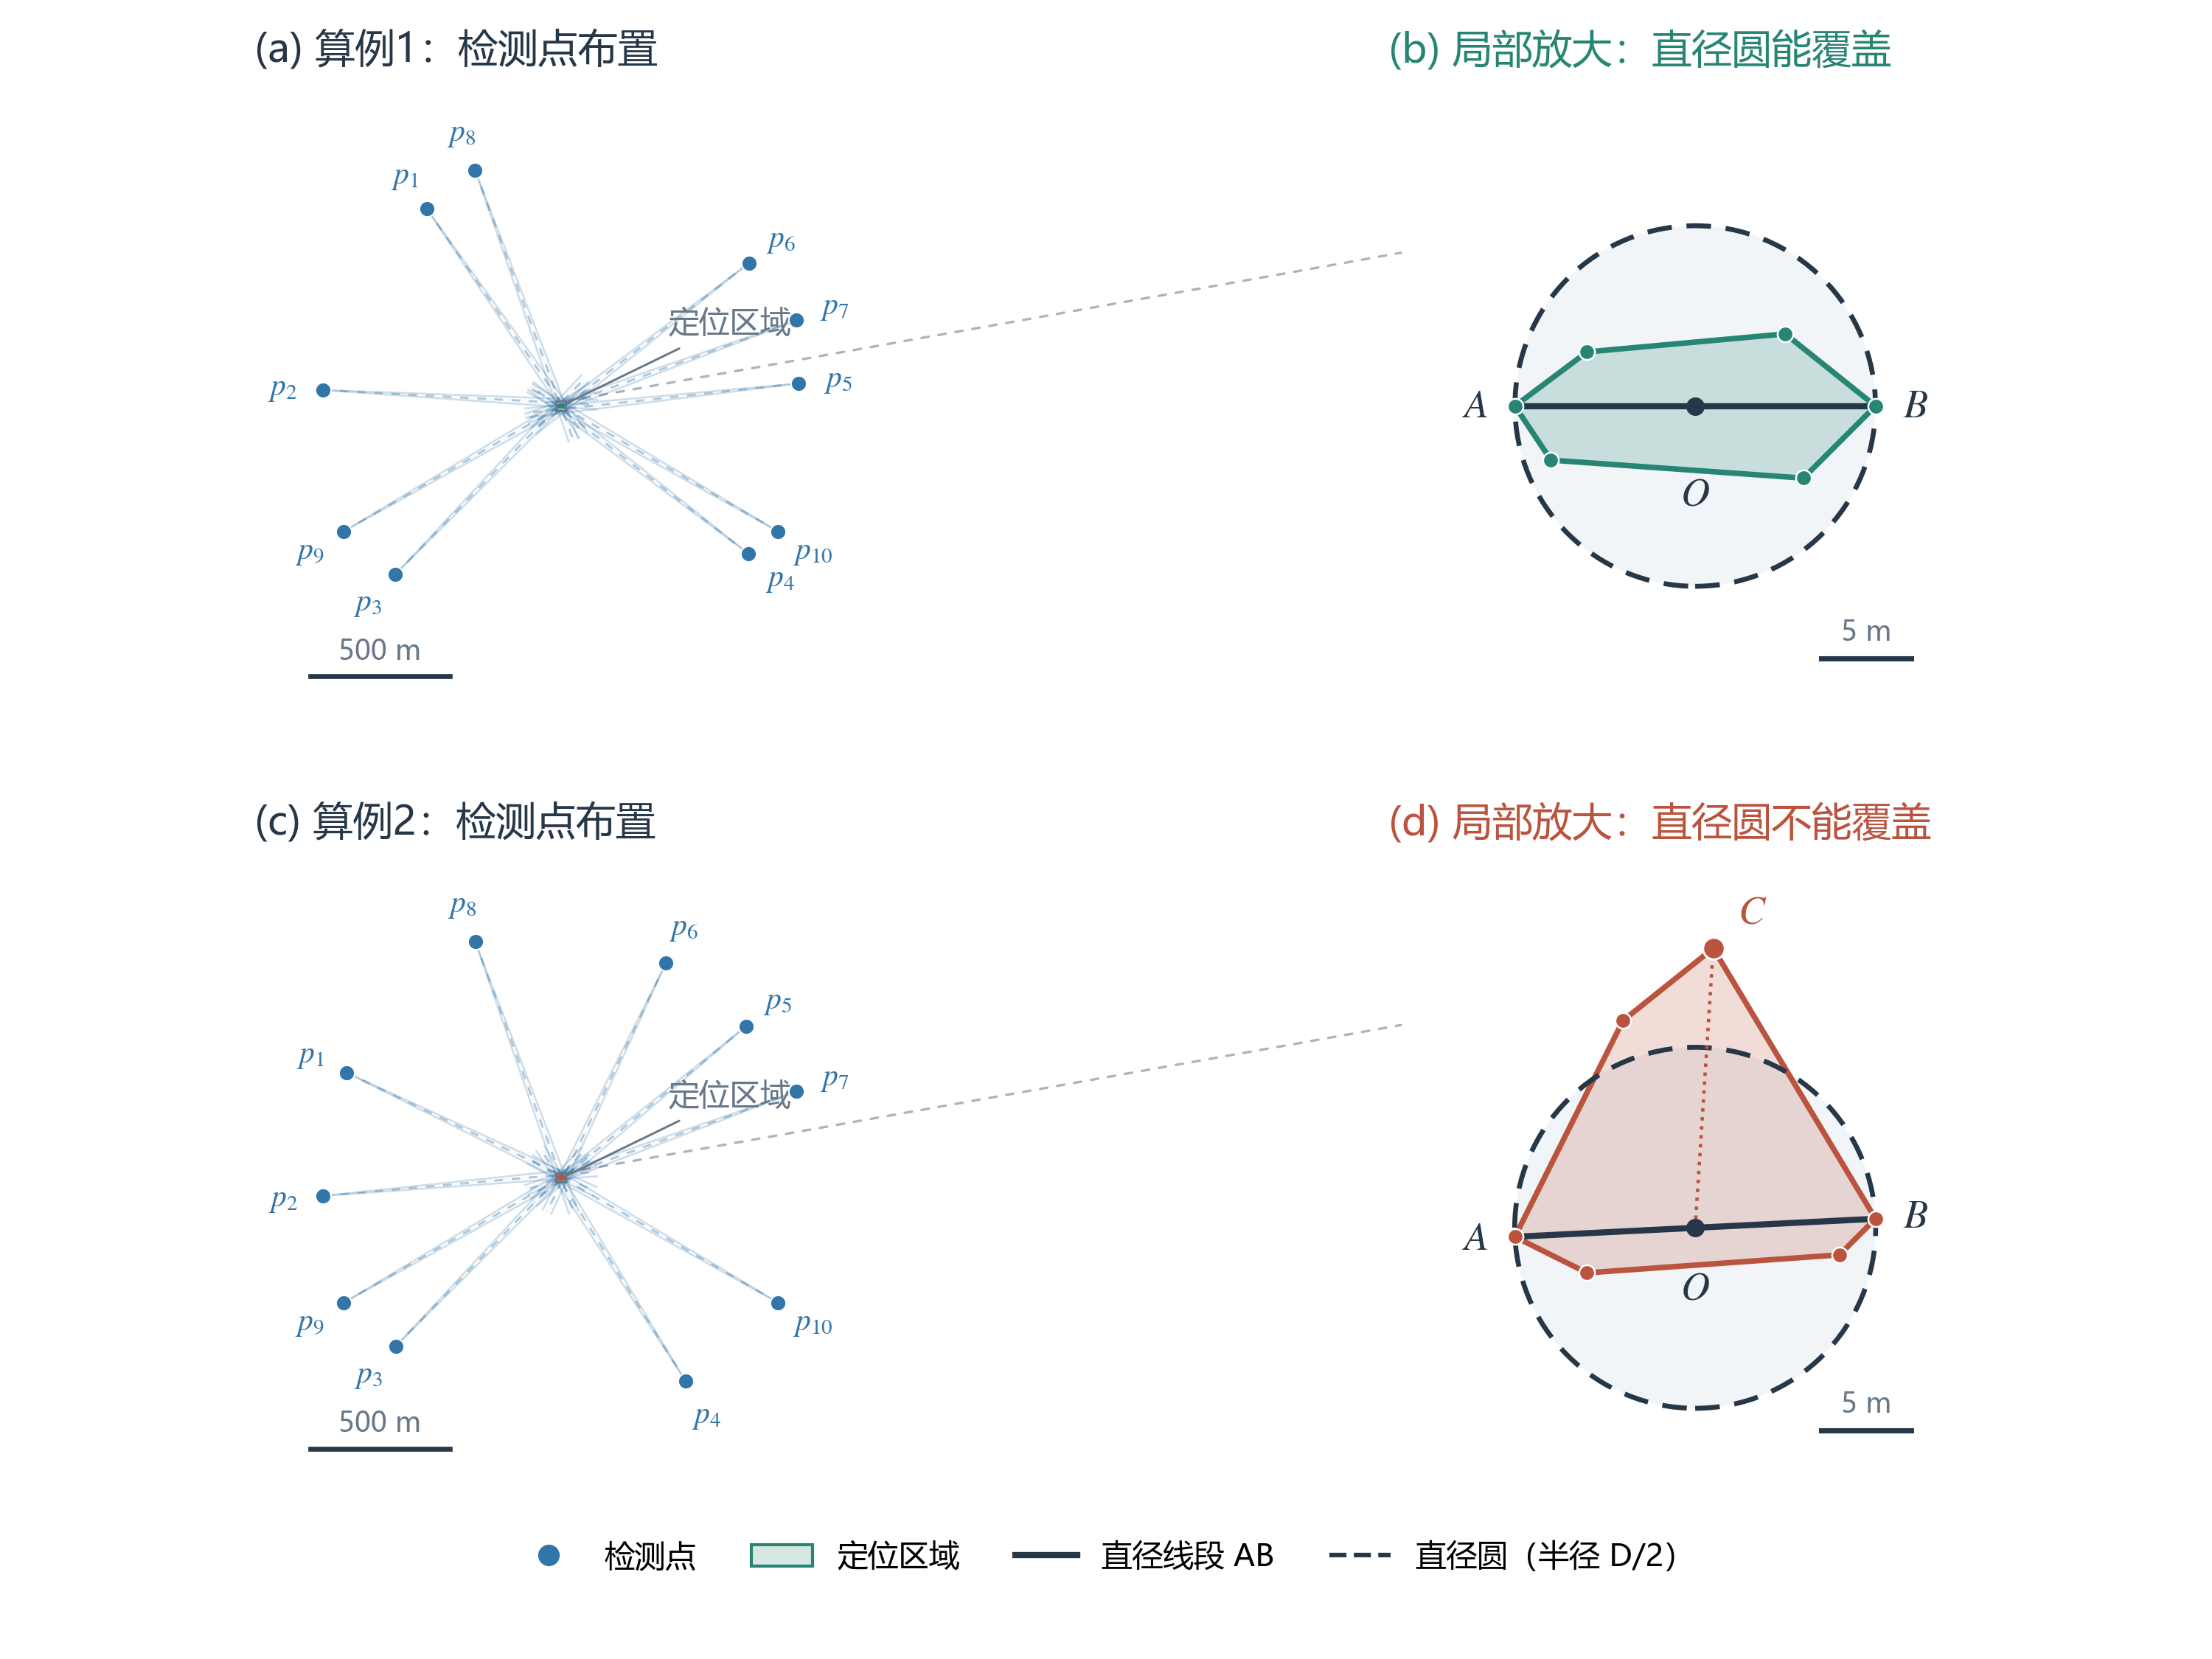
\includegraphics[width=0.94\linewidth]{data/q1_two_cases/q1_two_cases.png}
  \caption{两组算例的检测点布置、定位区域与直径圆}
  \label{fig:q1-experiment}
\end{figure}

% 数值与输入：data/q1_two_cases/results.json、case1_observations.csv、case2_observations.csv。
% 绘图与主算法：data/q1_two_cases/generate.py、geometry.py。
\label{sec:q1-end}


\subsection{问题二模型建立与求解}
\label{sec:q2}
% 本节沿用固定R0模型；表述与基线对照按第二问审查意见前五项整理。

\subsubsection{定位指标与选点准则}
\label{sec:q2-effect}

第一次测向通常留下沿示向方向延伸的狭长楔形区域。第二检测点的位置既影响两次测向的交会几何，
也影响能否接收到信号，因此选点时需同时考虑\textbf{观测后区域能缩小多少}与\textbf{各种反馈出现的概率}。
本问以第二次检测后的期望定位范围为依据，给出推荐测点及其附近的近优候选区域。

沿用第一问的\textbf{最小覆盖圆半径 $R_*$}评价定位范围。相比面积，该指标能够反映狭长区域
在最不确定方向上的尺度；以最小覆盖圆圆心作为位置估计时，$R_*$ 即全部可行位置对应的
最坏情况误差。区域直径保留为辅助指标。

对候选点 $\boldsymbol q$，记可能反馈的集合为 $\mathcal Y$，其中包括正常示向的角度档、
“距离过近”和“无信号”。记反馈 $y$ 的预测概率为 $\pi_y(\boldsymbol q)$，
反馈后的完整可行区域为 $P_2(\boldsymbol q,y)$，则选点评价函数为
\begin{equation}
  J(\boldsymbol q)=\sum_{y\in\mathcal Y}
    \pi_y(\boldsymbol q)R_*\!\left(P_2(\boldsymbol q,y)\right).
  \label{eq:q2-objective}
\end{equation}
概率用于综合尚未发生的观测结果，各反馈下的覆盖半径则描述相应的几何定位范围。
因此，$J$ 能够衡量给定概率模型下的平均定位效果。

在目标圆域内建立候选网格 $\mathcal G$，定义推荐点与近优候选集合为
\begin{equation}
  \begin{aligned}
    \boldsymbol q_*&\in\underset{\boldsymbol q\in\mathcal G}{\operatorname{argmin}}\,J(\boldsymbol q),\\
    \mathcal C_\eta&=\left\{\boldsymbol q\in\mathcal G:
    J(\boldsymbol q)\leq(1+\eta)J(\boldsymbol q_*)\right\}.
  \end{aligned}
  \label{eq:q2-candidate-set}
\end{equation}
下文取 $\eta=0.1$ 展示 $10\%$ 近优区域，表示允许期望覆盖半径相对推荐点增加不超过 $10\%$。
这一阈值是候选区域的选取约定。下面先建立首次观测后的位置信息，再给出反馈预测与数值计算方法。

\subsubsection{首次观测后的位置信息}
\label{sec:q2-bayes}

首先，由于\textbf{同一目标干扰源的发射功率及测向机的灵敏度确定}，本问针对同一目标干扰源进行的两次检测，将接收半径
$R_0\in[1000,1500]\,\mathrm m$ 当成\textbf{固定参数}进行处理，在两次检测及候选测点的比较中保持不变。
以下，在给定 $R_0$ 的条件下，固定第一检测点 $\boldsymbol p_1$ 及其正常示向度 $\theta_1$，
确定第二检测点。记圆形目标区域为 $\Omega$，则第一次观测后的可行区域为
\begin{equation}
  P_1=\Omega\cap W_1\cap
  \{\boldsymbol x:5<\|\boldsymbol x-\boldsymbol p_1\|_2\leq R_0\}.
  \label{eq:q2-first-region}
\end{equation}
式中三个约束分别\textbf{对应目标分布范围}、\textbf{示向度误差范围}和\textbf{正常测向的距离条件}。
其中，$W_1$ 由第一次示向度及其两侧各 $\varepsilon=1^\circ$ 的误差确定（楔形）；
目标圆域与距离条件进一步裁剪该楔形，所得 $P_1$ 构成第二次选点的初始区域。

依据第~\ref{sec:assumptions} 节的位置先验与测角误差假设，目标在 $\Omega$ 内按单位面积均匀分布，
首次测角误差在 $[-\varepsilon,\varepsilon]$ 内均匀分布。由此，各可行位置产生第一次示向度的
似然密度均为 $1/(2\varepsilon)$，经贝叶斯更新后，位置分布在 $P_1$ 内仍保持均匀。
因此，$P_1$ 内任一子区域的概率等于其面积占比。这一关系为位置离散后的概率赋值提供了依据。

\subsubsection{反馈预测与数值计算}
\label{sec:q2-numerics}

为计算式~\eqref{eq:q2-objective}，将位置积分、反馈预测和区域更新结合起来。
位置积分采用扇环单元，尚未获得的示向度采用角度分档；二者分别用于近似位置分布和反馈分布。
计算时，将圆形区域划分为小扇环，并保留与 $P_1$ 相交的部分。
用 $\ell$ 表示位置单元编号，$E_\ell$ 表示裁剪后的单元，
$\boldsymbol z_\ell$ 为其中的代表点，则该单元的概率权重为
\[
  w_\ell=\frac{\operatorname{Area}(E_\ell)}{\operatorname{Area}(P_1)},
  \qquad \sum_\ell w_\ell=1.
\]
\textbf{单元权重由实际面积确定}：只有等面积单元才具有相同概率，
等径向间距、等角度间距的扇环单元\textbf{仍需按面积加权}。
对边界单元，使用其与 $P_1$ 的交集面积；代表点用于近似单元内的积分，
在测角或距离边界附近进一步细分，以减小离散误差。

\begin{figure}[htbp]
  \centering
  \begin{minipage}[b]{0.48\linewidth}
    \centering
    \parbox[c][5.4cm][c]{\linewidth}{\centering
      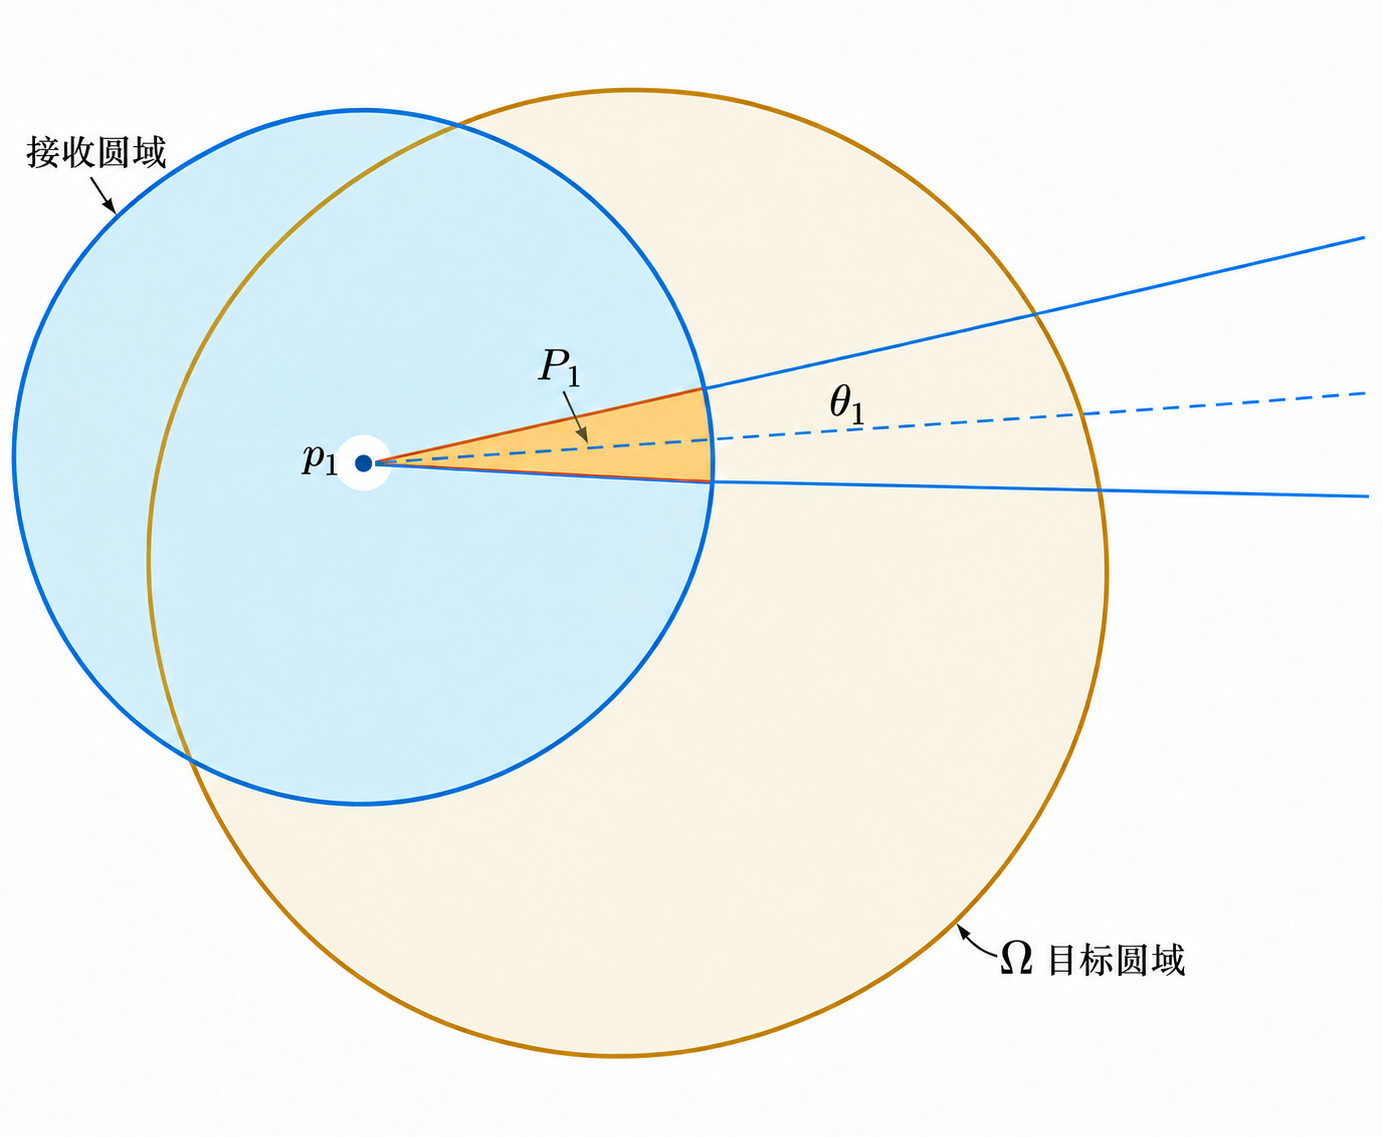
\includegraphics[width=\linewidth,height=5.2cm,keepaspectratio]{data/q2_initial_region_v1/q2_initial_region_v1.png}}
    \par\smallskip
    {\small (a) 初始可行区域}
  \end{minipage}\hfill
  \begin{minipage}[b]{0.48\linewidth}
    \centering
    \parbox[c][5.4cm][c]{\linewidth}{\centering
      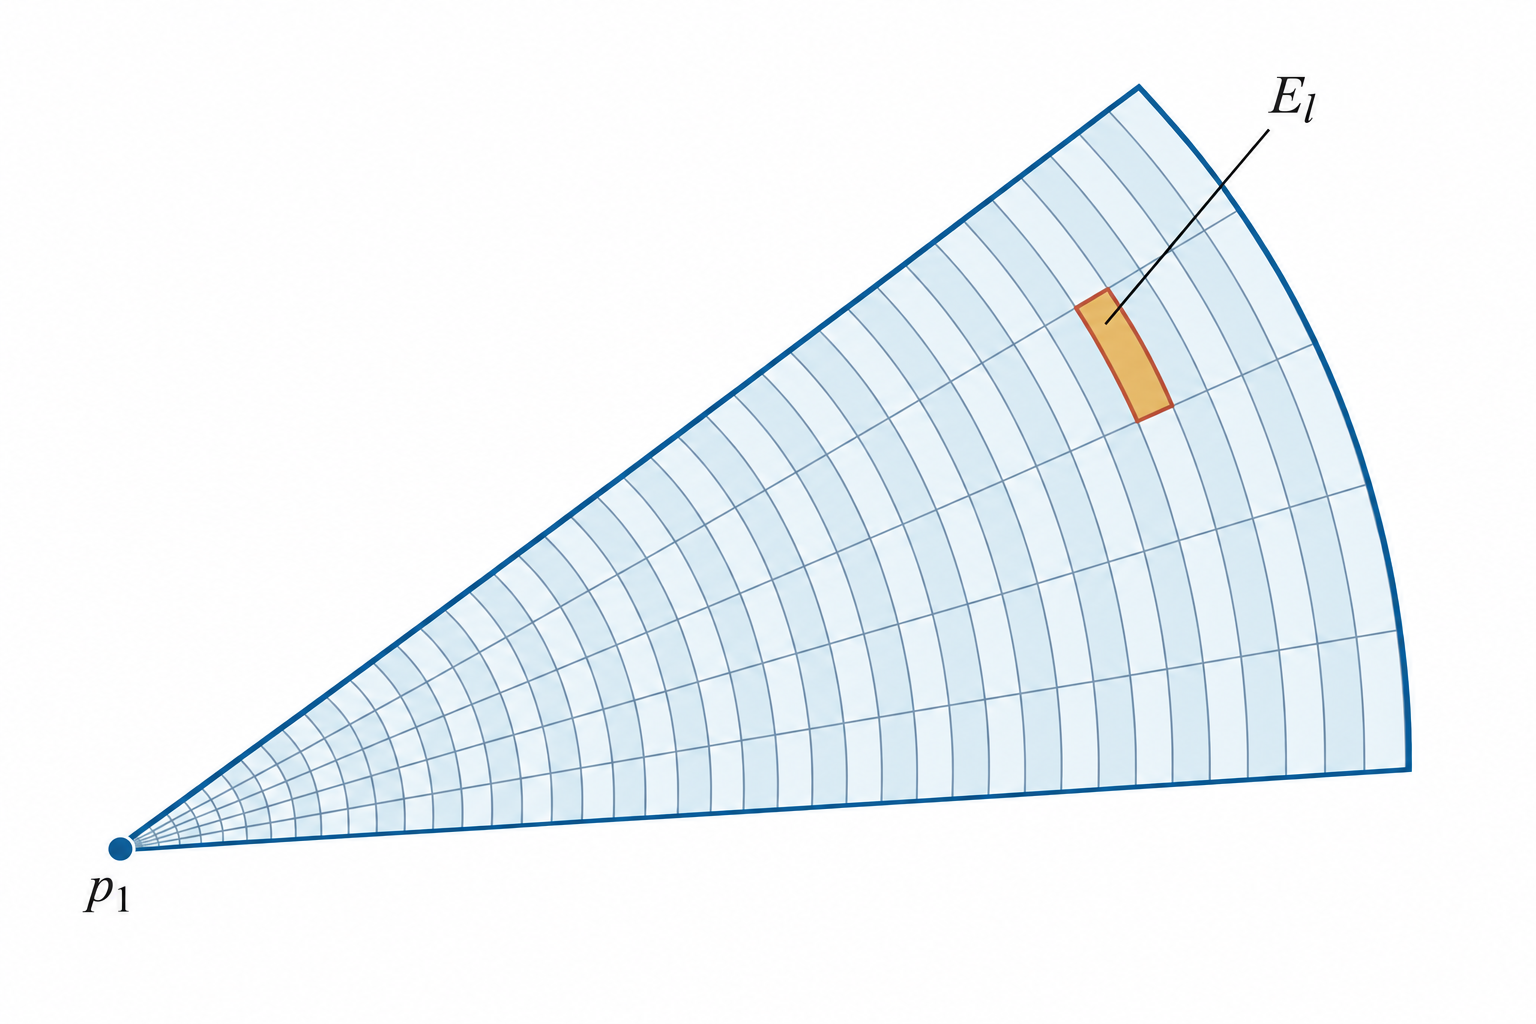
\includegraphics[width=\linewidth,height=5.2cm,keepaspectratio]{data/q2_annular_grid_v3/q2_annular_grid_v3.png}}
    \par\smallskip
    {\small (b) 扇环离散示意}
  \end{minipage}
  \caption{初始可行区域与位置离散（误差角及近距离排除区域放大示意）}
  \label{fig:q2-discretization}
\end{figure}

对候选第二检测点 $\boldsymbol q$，记代表位置 $\boldsymbol z_\ell$ 相对该测点的
距离和真实方位分别为 $d_\ell(\boldsymbol q)$、$\varphi_\ell(\boldsymbol q)$。
根据测向机的工作条件，第二次检测包含三类反馈：距离不超过 $5\,\mathrm m$ 时返回
“距离过近”，超过 $R_0$ 时返回“无信号”，其余情形返回带有误差的示向度。
三类反馈共同构成选点评价所需的完整观测空间，不能只考虑成功返回示向度的情形。

实际获得第二次示向度后，直接以该读数为中心构造\textbf{总张角为 $2^\circ$ 的楔形}，
与已有可行区域及距离约束求交即可。
但选点时读数尚未确定，为计算期望，将 $[0,2\pi)$ 划分为互不重叠的角度档 $B_h$。
在均匀误差假设下，第 $\ell$ 个位置单元产生第 $h$ 档反馈的概率，
可由代表点的读数范围与该档的重叠角长占比近似计算：
\begin{equation}
  L_{\ell h}(\boldsymbol q)\approx
  \operatorname{Bool}\!\left(5<d_\ell(\boldsymbol q)\leq R_0\right)
  \frac{\left|B_h\cap
  [\varphi_\ell(\boldsymbol q)-\varepsilon,\,
   \varphi_\ell(\boldsymbol q)+\varepsilon]\right|_{\mathrm{circ}}}{2\varepsilon}.
  \label{eq:q2-likelihood}
\end{equation}
其中，$\operatorname{Bool}(\cdot)$ 为布尔型函数，在括号内条件成立时取 $1$，否则取 $0$；
$|\cdot|_{\mathrm{circ}}$ 为圆周角长。“距离过近”和“无信号”的概率由相应距离条件确定，
三类反馈的概率之和为 $1$。\textbf{角度分档仅用于选点前的期望计算，不改变实测后的两度楔形。}

\begin{figure}[htbp]
  \centering
  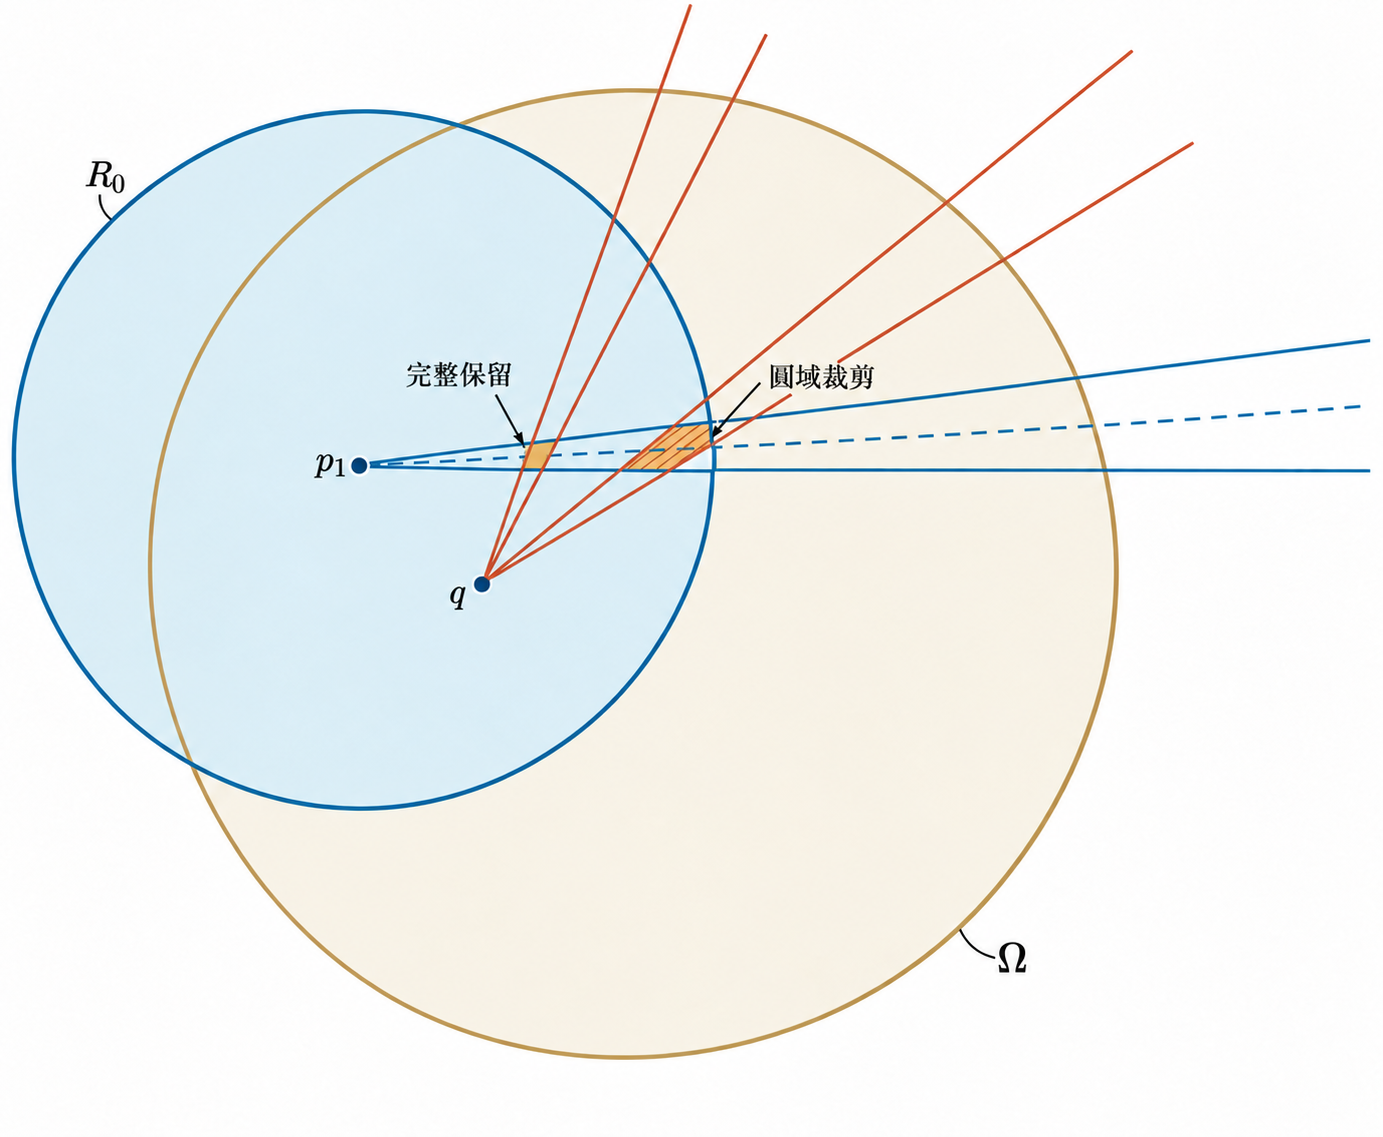
\includegraphics[width=0.6\linewidth]{data/q2_reception_clipping_v4/q2_reception_clipping_v4.png}
  \caption{不同第二示向度下的可行区域更新（误差角放大示意）}
  \label{fig:q2-prediction}
\end{figure}

图~\ref{fig:q2-prediction} 中，两组示向边界表示同一候选测点处的两种可能反馈，
分别与初始区域求交，而非同时施加约束；图示仅说明区域更新，反馈概率由式~\eqref{eq:q2-likelihood} 计算。

用 $\mathcal Y$ 表示包含各角度档、“距离过近”和“无信号”的反馈集合。
根据全概率公式和贝叶斯公式，反馈 $y$ 的预测概率与反馈后的单元权重分别为
\begin{equation}
  \pi_y(\boldsymbol q)=\sum_\ell w_\ell L_{\ell y}(\boldsymbol q),\qquad
  w_{\ell\mid y}(\boldsymbol q)
  =\frac{w_\ell L_{\ell y}(\boldsymbol q)}{\pi_y(\boldsymbol q)}.
  \label{eq:q2-bayes}
\end{equation}
前式对所有可能位置加权求和，得到选点时所需的反馈分布；
后式在给定反馈后更新位置概率，排除不相容的位置，并调整其余单元的相对权重。
其中，后验更新仅对 $\pi_y(\boldsymbol q)>0$ 的反馈进行，
预测分布满足 $\sum_{y\in\mathcal Y}\pi_y(\boldsymbol q)=1$。

与概率更新相对应，记反馈后的\textbf{完整可行区域}为 $P_2(\boldsymbol q,y)$。
对于具体示向度，该区域由 $P_1$ 与第二楔形及正常测向距离范围相交得到。
在角度分档计算中，一档包含多个可能的示向度，应取这些示向度对应楔形的并集。
对于宽度为 $\Delta\theta$ 的窄角度档，该并集等价于以档中心为方向、
半张角为 $\varepsilon+\Delta\theta/2$ 的楔形。
其中增加的 $\Delta\theta/2$ 用于保留分档所包含的角度不确定性，并随档宽减小而趋于零。

对于“距离过近”，$P_2$ 为 $P_1$ 与以 $\boldsymbol q$ 为圆心、半径 $5\,\mathrm m$
的圆盘的交集，其最小覆盖圆半径不超过 $5\,\mathrm m$；
对于“无信号”，$P_2$ 为 $P_1$ 中距离 $\boldsymbol q$ 超过 $R_0$ 的部分。
两类反馈均通过\textbf{距离约束}更新可行区域，其定位效果同样由更新后区域的覆盖半径评价。

将得到的反馈概率与区域覆盖半径代入式~\eqref{eq:q2-objective}，即可计算各候选点的 $J$，
并按式~\eqref{eq:q2-candidate-set} 确定推荐点与候选区域。

按题设，同一位置重复检测的读数不变，故第一检测点可以单独取
$J(\boldsymbol p_1)=R_*(P_1)$。

下文位置积分采用 $80\times16$ 个扇环单元，示向度档宽为 $0.125^\circ$。
候选网格间距为 $60\,\mathrm m$，在粗网格最佳点附近的 $\pm90\,\mathrm m$ 范围内加密至
$15\,\mathrm m$；对称情形同时考察镜像邻域。推荐坐标与目标值均对应这一离散计算设置。

\subsubsection{结果可视化与策略比较}
\label{sec:q2-experiment}

为考察初始几何关系对第二检测点选择的影响，我们设置了对称与不对称两组情形。
目标圆域半径均取 $1800\,\mathrm m$，接收半径固定为 $R_0=1200\,\mathrm m$，
测角误差半宽为 $1^\circ$。对称情形取 $\boldsymbol p_1=(0,0)\,\mathrm m$、
初次示向度 $0^\circ$；不对称情形取 $\boldsymbol p_1=(1200,400)\,\mathrm m$、
初次示向度 $65^\circ$。下面先展示推荐区域，再用一个构造情形呈现交会结果，
最后比较不同选点策略的期望定位效果。

\textbf{推荐测点与候选区域。}图~\ref{fig:q2-experiment} 展示两组情形的期望覆盖半径。
两图共用对数色标，颜色由紫色经蓝绿色趋向黄色时，$J$ 逐渐减小。
星标为网格搜索得到的推荐点，虚线为式~\eqref{eq:q2-candidate-set} 中
$\eta=0.1$ 所对应阈值的网格插值等值线，用于展示近优区域。
颜色块对应实际网格计算值，虚线用于可视化；推荐点不代表连续区域内的严格全局最优解。

\begin{figure}[htbp]
  \centering
  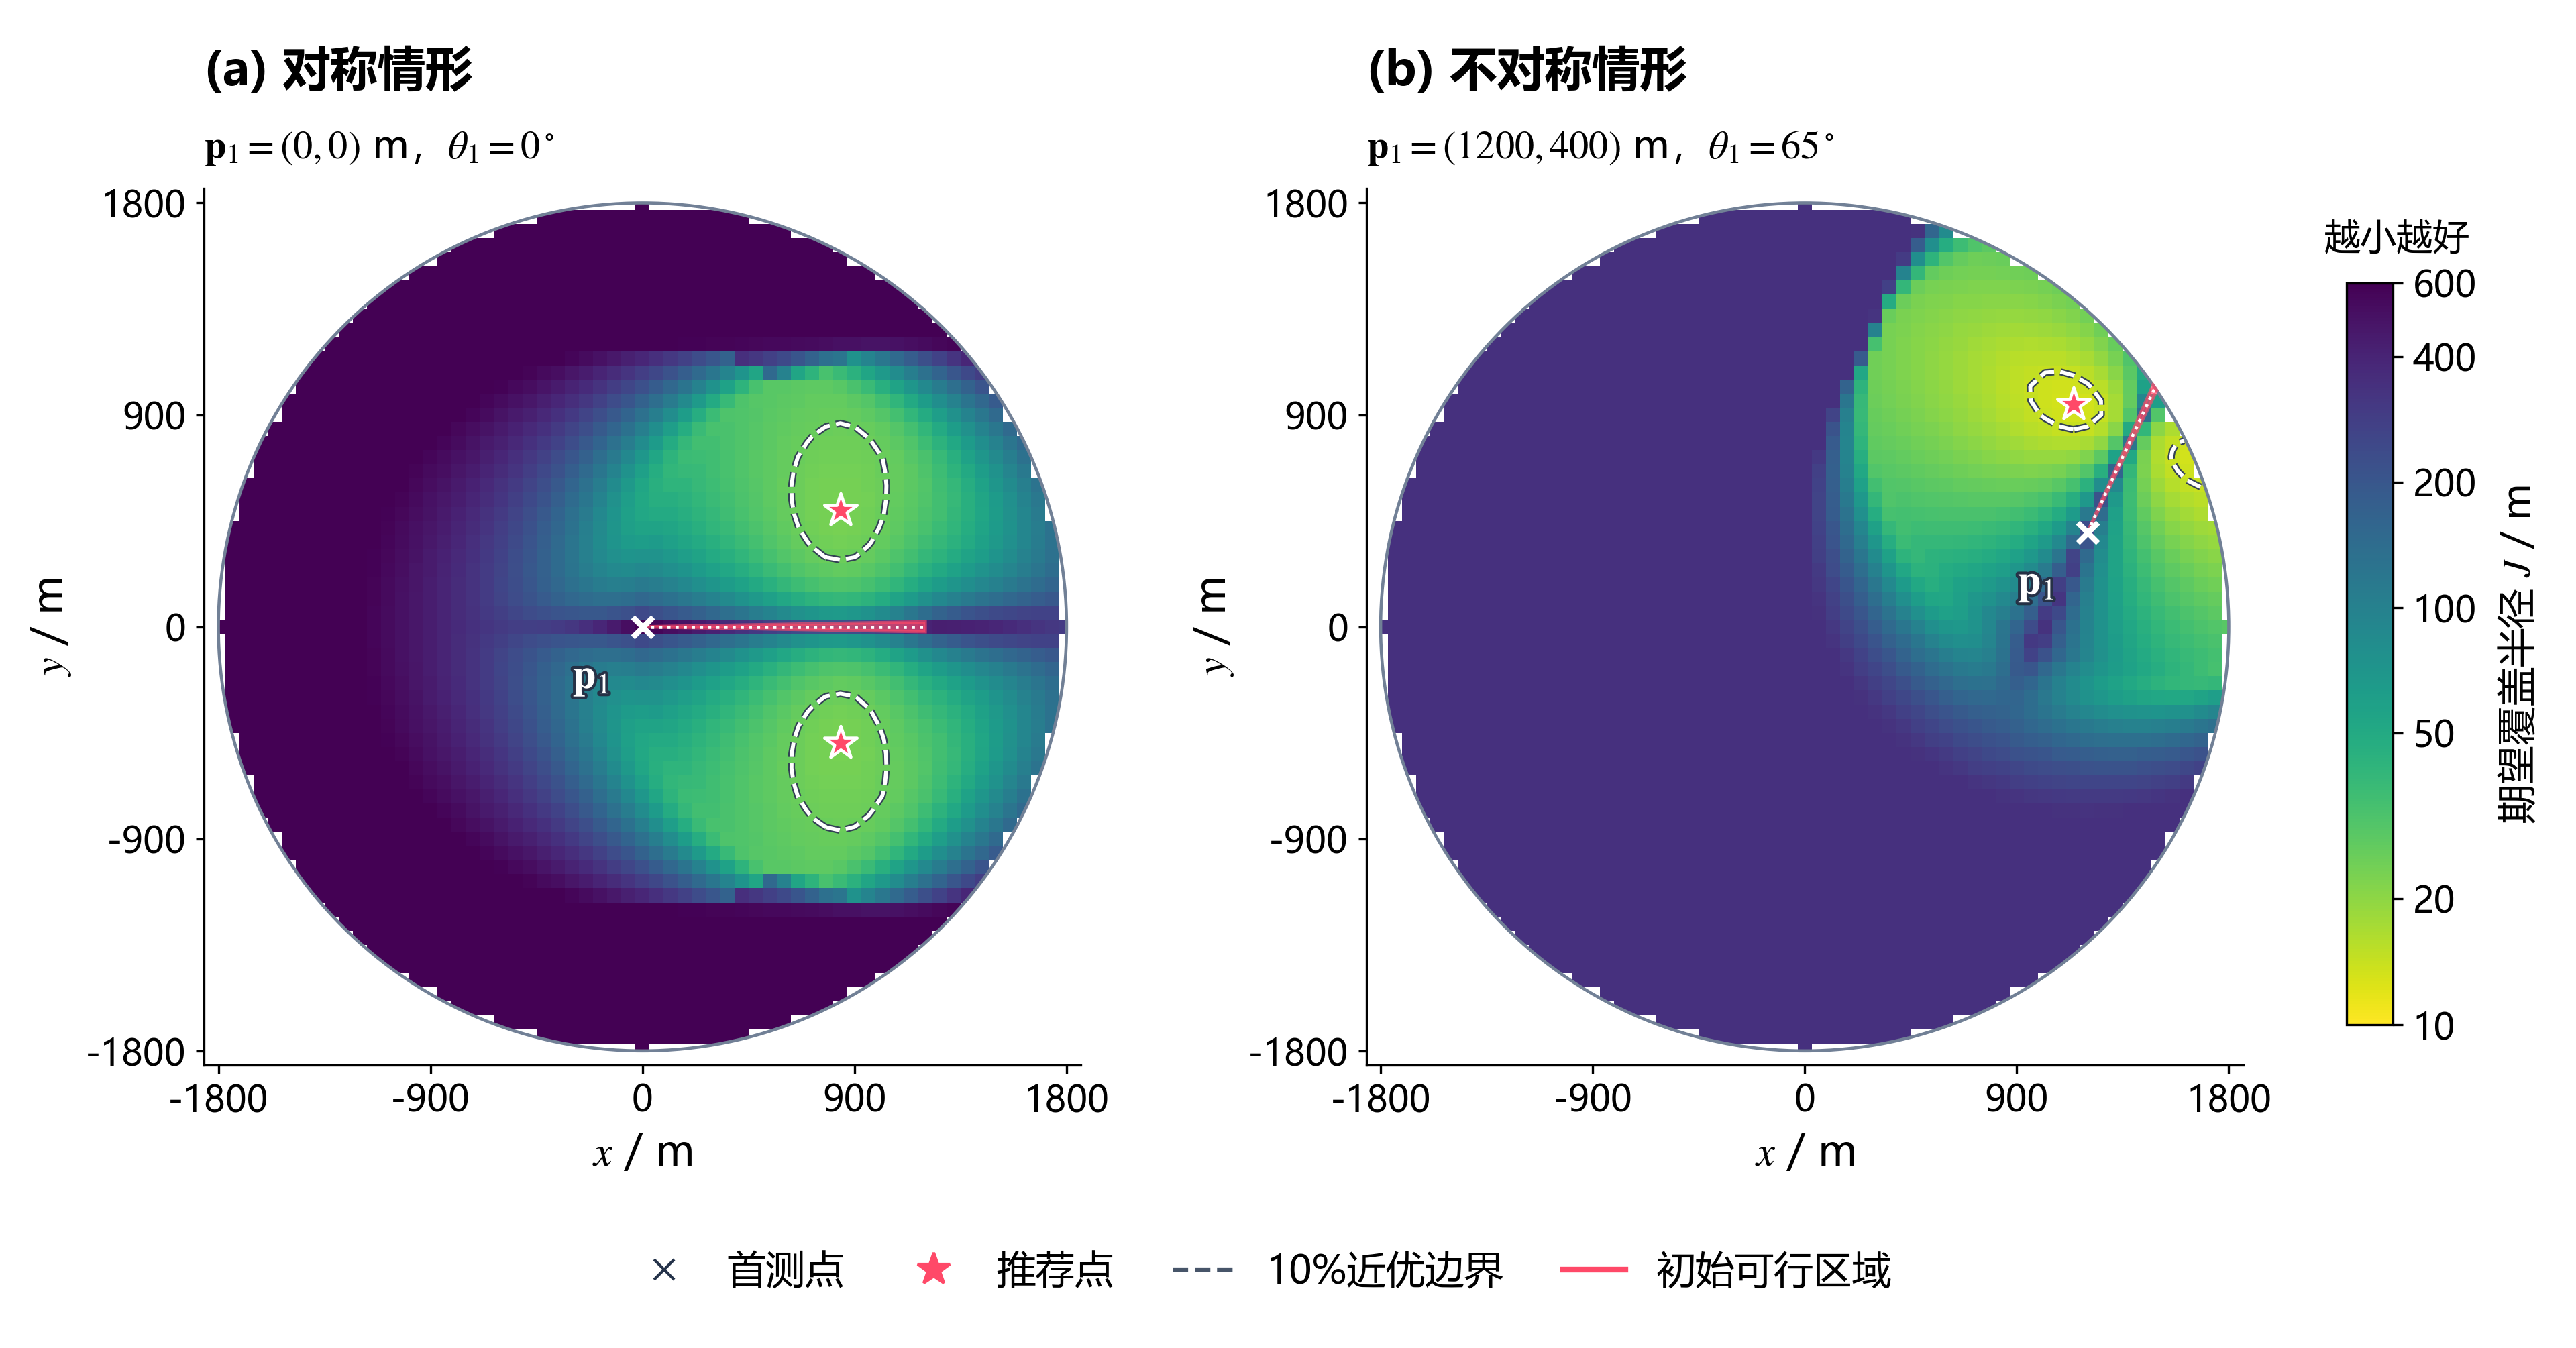
\includegraphics[width=\linewidth]{data/q2_strategy_heatmaps/q2_strategy_heatmaps.png}
  \caption{两组初始条件下的推荐测点及近优候选区域（共用对数色标）}
  \label{fig:q2-experiment}
\end{figure}

对称情形下，目标圆域、首测点及首次楔形均关于 $x$ 轴对称，位置先验和误差模型
也保持这一对称性，故上下镜像测点的 $J$ 相同，推荐点为 $(840,\pm495)\,\mathrm m$。
不对称情形中，目标圆域的裁剪打破了关于首示向线的对称性，
推荐点变为 $(1140,945)\,\mathrm m$，需依据裁剪后的初始区域重新选点。

\textbf{不同选点下的交会结果。}为直观展示第二次观测带来的区域变化，
以沿首示向前进 $300\,\mathrm m$、朝其左侧垂直方向移动 $300\,\mathrm m$
作为两种简单选点策略，与推荐点比较。
在对称情形中构造源位置 $\boldsymbol s=(900,0)\,\mathrm m$，首次测角误差取 $0^\circ$，
三种第二测点的测角误差均取 $+0.35^\circ$，均返回正常示向。
根据上述区域更新算法，得到图~\ref{fig:q2-intersection-comparison} 所示的交会区域及最小覆盖圆。

\begin{figure}[!htb]
  \centering
  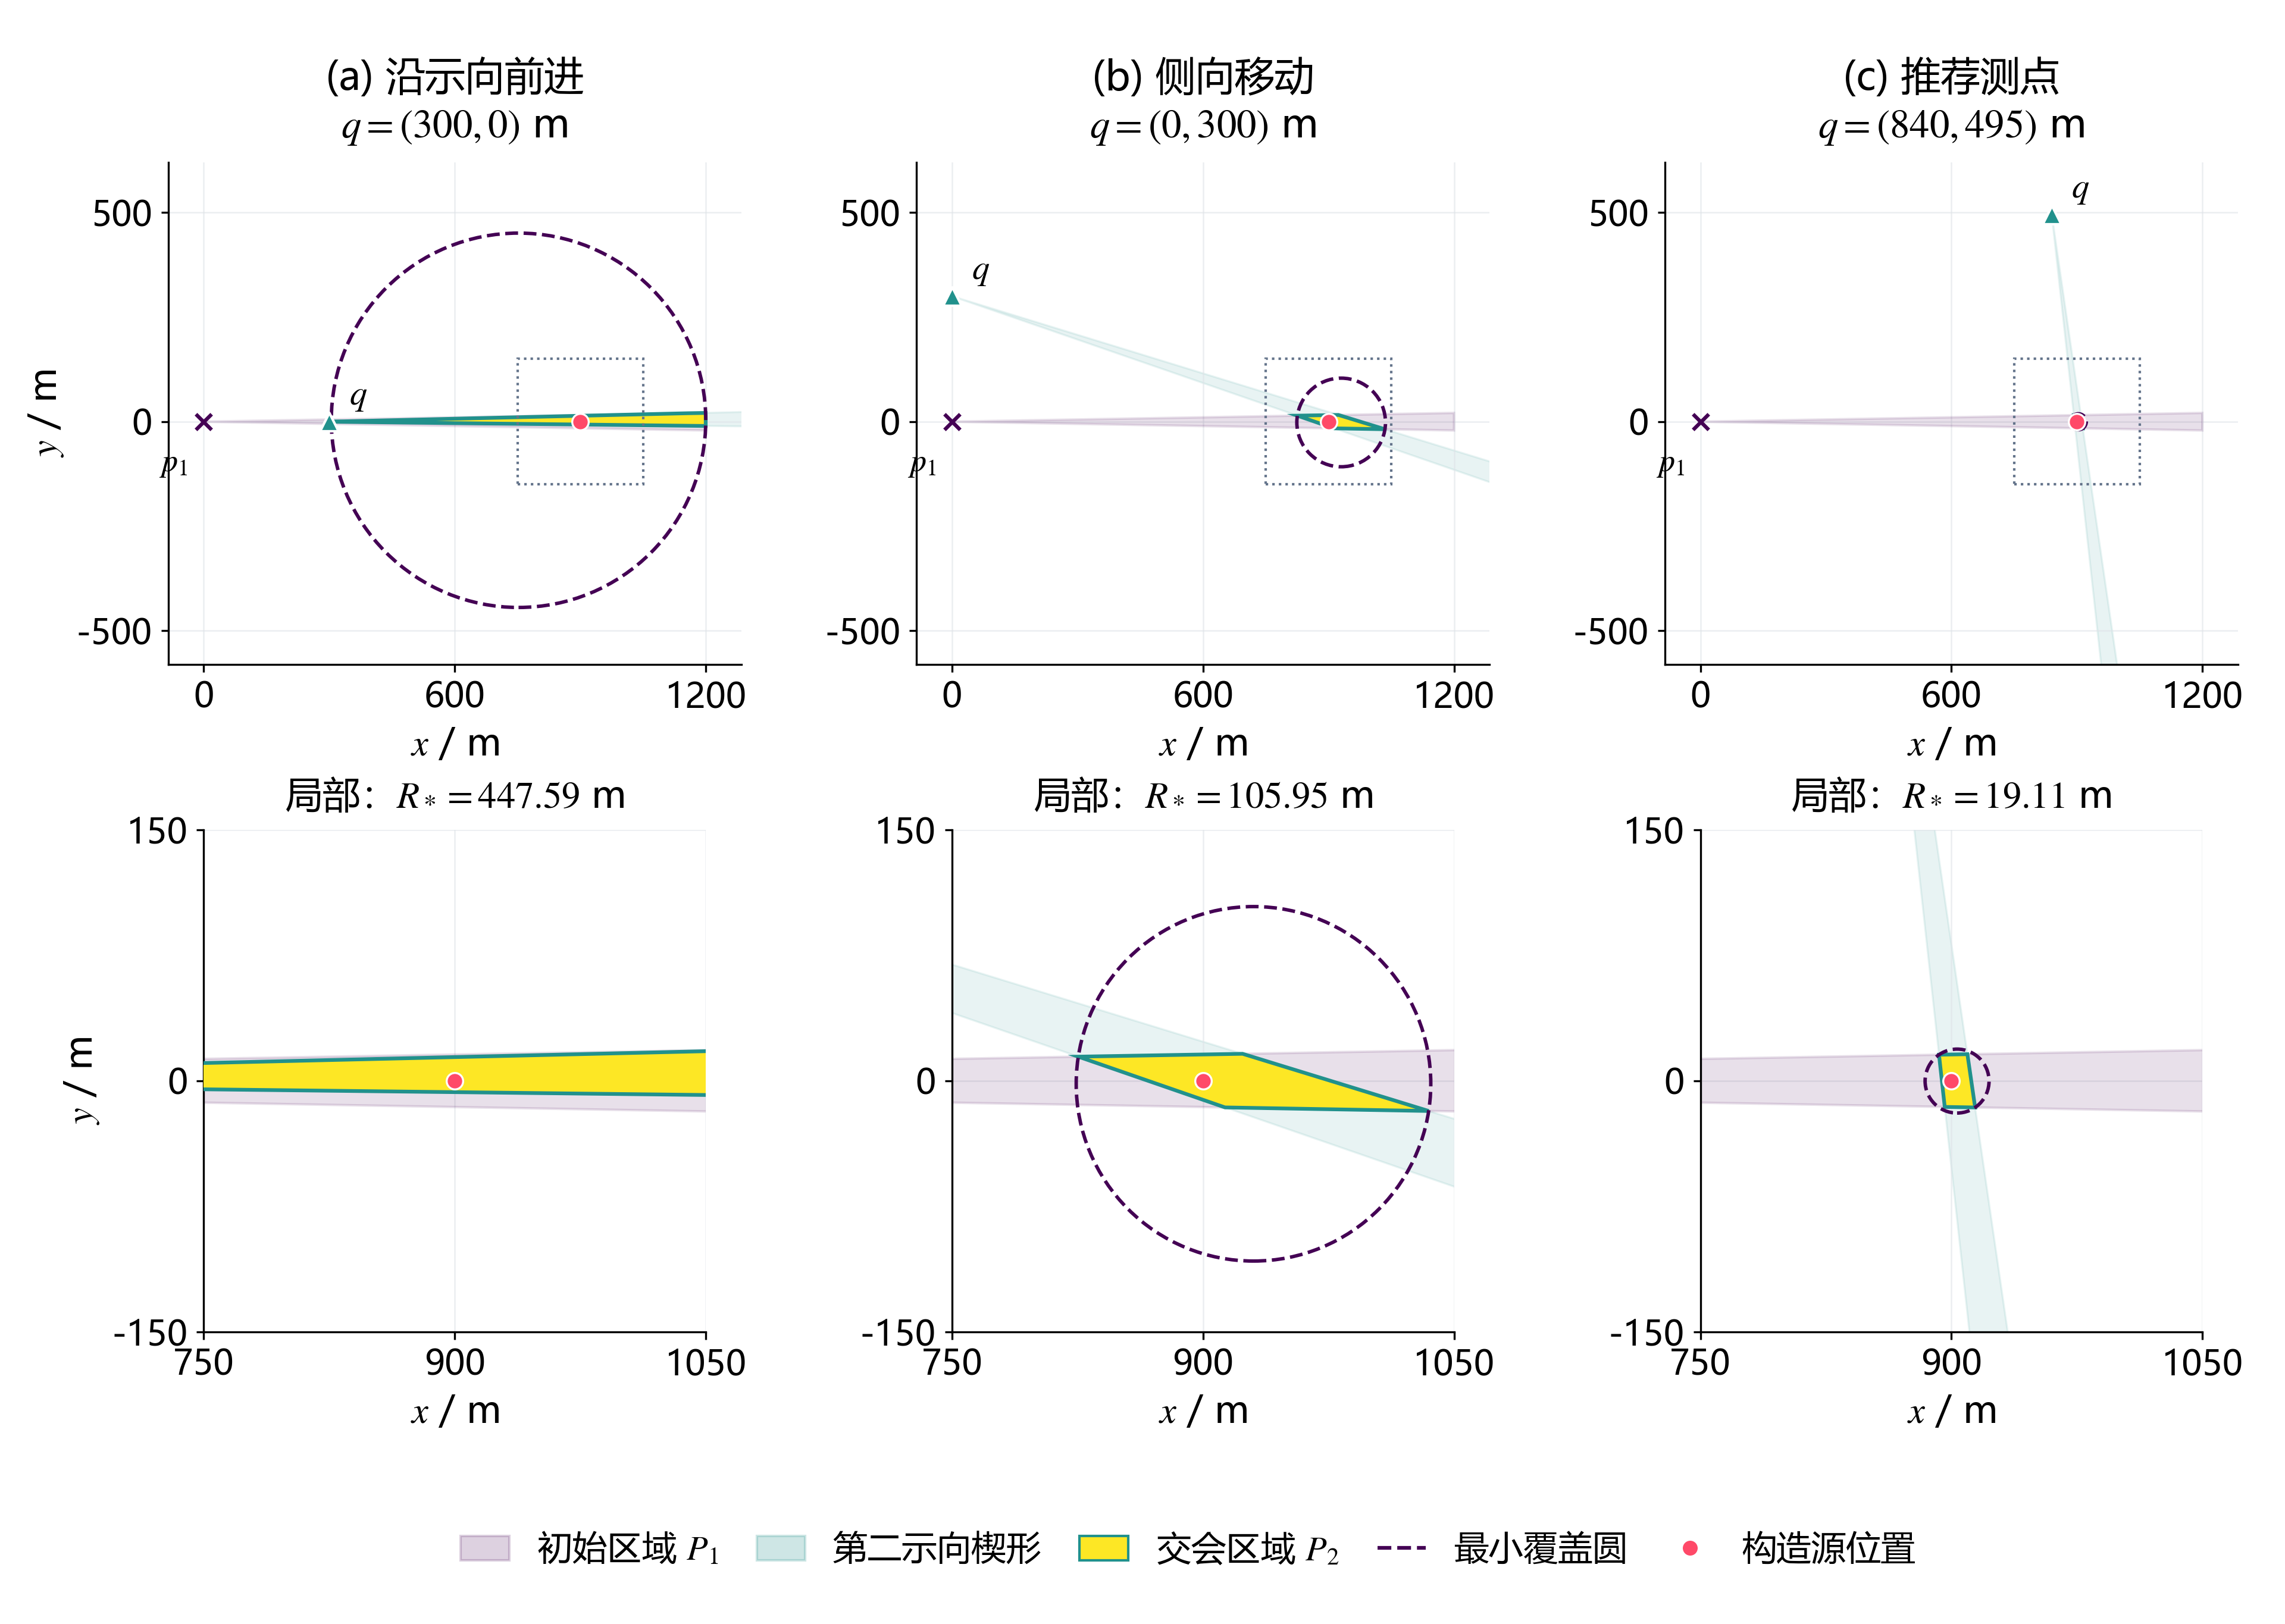
\includegraphics[width=\linewidth]{data/q2_intersection_comparison/q2_intersection_comparison.png}
  \caption{三种第二测点下的交会结果：上排为整体位置关系，下排为虚框内的局部放大}
  \label{fig:q2-intersection-comparison}
  \par\smallskip
  \parbox{0.96\linewidth}{\footnotesize 注：各列的整体视图采用相同坐标范围，局部视图也采用相同坐标范围。
  左下图的覆盖圆超出局部窗口，其完整形状见左上图。该图展示固定构造情形的单次结果，图中半径不是期望值 $J$。}
\end{figure}

\begin{samepage}
这一构造情形中，初始覆盖半径为 $597.59\,\mathrm m$。
沿示向前进后，两次楔形接近同向，交会区域仍然狭长，覆盖半径为 $447.59\,\mathrm m$；
侧向移动后，第二楔形从不同方向切割初始区域，覆盖半径降至 $105.95\,\mathrm m$；
在推荐点观测后，覆盖半径为 $19.11\,\mathrm m$。
这些结果用于展示区域收缩的几何过程，策略的平均效果仍由各类反馈加权后的 $J$ 评价。
\par
\end{samepage}

\textbf{期望定位效果比较。}表~\ref{tab:q2-baselines} 将测点坐标、期望覆盖半径和无信号概率
集中列出，两组初始覆盖半径分别为 $597.59\,\mathrm m$ 和 $340.22\,\mathrm m$。
所有期望值均采用前述相同数值参数计算。

\begin{table}[!htb]
  \centering
  \caption{推荐测点与简单选点策略的期望定位效果}
  \label{tab:q2-recommendations}
  \label{tab:q2-baselines}
  \small
  \setlength{\tabcolsep}{5pt}
  \renewcommand{\arraystretch}{1.15}
  \begin{tabular}{llcrr}
    \toprule
    情形 & 选点策略 & 测点坐标/m & $J$/m & 无信号概率/\% \\
    \midrule
    对称 & 沿示向前进 & $(300,0)$ & 409.03 & 0.00 \\
         & 侧向移动 & $(0,300)$ & 72.74 & 6.25 \\
         & 推荐点 & $(840,\pm495)$ & 23.15 & 0.00 \\
    \midrule
    不对称 & 沿示向前进 & $(1326.79,671.89)$ & 157.36 & 0.00 \\
           & 侧向移动 & $(928.11,526.79)$ & 31.15 & 0.00 \\
           & 推荐点 & $(1140,945)$ & 12.93 & 0.00 \\
    \bottomrule
  \end{tabular}
  \par\smallskip
  \parbox{0.96\linewidth}{\footnotesize 注：两种简单策略均相对首测点移动 $300\,\mathrm m$；
  $\pm$ 表示一对镜像推荐点。坐标按显示精度取舍，计算使用未舍入坐标。
  无信号概率为位置求积近似值。本表比较定位范围，各策略移动距离不同，未计移动时间。}
\end{table}
% 期望指标沿用 src/Q2/results/paper_baselines/results.json；构造交会结果见 data/q2_intersection_comparison/。

两组情形中，侧移策略的 $J$ 均小于沿示向前进策略；进一步选择前方侧向的推荐点后，
相比侧移 $300\,\mathrm m$，两组 $J$ 分别降低约 $68.2\%$ 和 $58.5\%$。
这一比较综合了可能的第二次反馈，与图~\ref{fig:q2-intersection-comparison} 的单次交会结果相互补充。

选点还受到接收范围的制约。例如，对称情形的侧移测点有约 $6.25\%$ 的无信号概率，
原因是初始区域远端的一部分位置距该测点超过 $R_0$。推荐点则兼顾交会几何与接收条件，
因此应结合整个初始区域比较各种反馈，而不能只依据某个假定源位置的交会角选点。
\FloatBarrier


\subsubsection{给定接收半径下的尺度变化}
\label{sec:q2-scale}

为说明给定接收半径如何改变推荐点和定位范围的尺度，在对称情形下固定
$\boldsymbol p_1=(0,0)\,\mathrm m$、初次示向度 $0^\circ$
及测角误差半宽 $1^\circ$，在题设允许的 $[1000,1500]\,\mathrm m$ 范围内，
以 $100\,\mathrm m$ 为间隔选取六组接收半径 $R_0$，比较第二检测点的选择结果。
目标圆域半径仍为 $1800\,\mathrm m$，每组实验均按相应的 $R_0$ 更新初始可行区域，
并按上述数值设置重新搜索第二检测点。利用镜像对称性，仅搜索上半圆域，
并核验对应镜像点的期望值一致。

\begin{table}[htbp]
  \centering
  \caption{给定接收半径下推荐点与期望定位范围的尺度变化}
  \label{tab:q2-r0}
  \small
  \setlength{\tabcolsep}{7pt}
  \renewcommand{\arraystretch}{1.25}
  \begin{tabular}{ccrrr}
    \toprule
    \shortstack{接收半径\\$R_0$/m} &
    \shortstack{推荐第二检测点\\$(x_2,y_2)$/m} &
    \shortstack{初始半径\\$R_*(P_1)$/m} &
    \shortstack{期望最小覆盖\\圆半径 $J$/m} &
    \shortstack{半径降幅\\/\%} \\
    \midrule
    1000 & $(705,\,\pm 420)$ & 497.6 & 19.3 & 96.1 \\
    1100 & $(765,\,\pm 450)$ & 547.6 & 21.2 & 96.1 \\
    1200 & $(840,\,\pm 495)$ & 597.6 & 23.1 & 96.1 \\
    1300 & $(900,\,\pm 540)$ & 647.6 & 25.1 & 96.1 \\
    1400 & $(975,\,\pm 585)$ & 697.6 & 27.0 & 96.1 \\
    1500 & $(1050,\,\pm 615)$ & 747.6 & 28.9 & 96.1 \\
    \bottomrule
  \end{tabular}
  \par\smallskip
  \parbox{0.94\linewidth}{\footnotesize 注：$\pm$ 表示一对镜像推荐点；$J$ 为各组网格搜索所得的最小期望值，
  半径降幅为 $[1-J/R_*(P_1)]\times100\%$。}
\end{table}

表~\ref{tab:q2-r0} 中，推荐点随 $R_0$ 增大而外移，且归一化坐标
$x_2/R_0$ 约为 $0.692$--$0.705$，$|y_2|/R_0$ 约为 $0.409$--$0.420$，
$J/R_0$ 均约为 $0.0193$，表现出近似的尺度关系。
本组首测点位于圆心且 $R_0<1800\,\mathrm m$，初始区域未受目标圆域外边界裁剪；
除固定的 $5\,\mathrm m$ 近距离排除范围外，几何尺度主要随 $R_0$ 同步变化。
这一关系不宜直接推广到受圆域边界裁剪的其他初始条件。

各组相对初始半径的降幅均约为 $96.1\%$，但绝对期望半径随 $R_0$ 增大，
不能据此解释为接收能力增强使定位变差，因为首次正常测向对应的条件位置分布也发生了变化。
本表展示分别给定 $R_0$ 时的尺度变化。

此外，将位置积分加密至 $160\times32$、示向度档宽减半，并加密圆弧近似后，
在各组原推荐点处重算的期望值变化均不超过 $1.3\%$。这一检查支持表中固定测点目标值的数值稳定性。

\subsection{问题三模型建立与求解}
\label{sec:q3}
% 框架暂按独立 Bayes 算法三组织。B3.2 原版与 Bayes 在现有代码中为不同策略，版本名称待统一。

问题二讨论了单个干扰源的第二检测点选择，而问题三需要在源数、频道、位置及接收半径
均未知的条件下完成全部清除。此时，定位精度只是决策的一部分：为了获得较好的交会角
而增加的移动，可能抵消少量检测带来的收益；清除已发现的源后，也仍需确认是否存在遗漏。
因此，我们在前两问的几何定位基础上，采用\textbf{Bayes 更新与动态路径规划相结合的策略}，
将后续检测、源的清除和未知频道搜索纳入同一时间评价。

\subsubsection{任务描述与评价目标}

沿用目标圆域 $\Omega$ 及前文的几何记号，以频道编号 $c$ 区分各干扰源。
同一频道至多对应一个源，其接收半径 $R_c\in[1000,1500]\,\mathrm m$ 在一次任务中保持不变。
机器狗从原点出发，初始频道为 $1$，每次只能在停止移动后检测一个频道。
我们将任务目标表述为：\textbf{在确认全部干扰源已清除的前提下，尽量减少总虚拟时间}。
按实际动作计费，总时间可分解为
\begin{equation}
  T=\frac{L}{5}+n_{\mathrm{sw}}+5n_{\mathrm{meas}}
    +5n_{\mathrm{succ}}+3n_{\mathrm{fail}}.
  \label{eq:q3-time}
\end{equation}
其中，$L$ 为总移动路程，$n_{\mathrm{sw}}$、$n_{\mathrm{meas}}$ 分别为实际切频与检测次数，
$n_{\mathrm{succ}}$、$n_{\mathrm{fail}}$ 为成功和失败的清除尝试次数。
成功清除包括 $3\,\mathrm s$ 光学定位与 $2\,\mathrm s$ 激光清除，失败尝试仅计光学定位时间。
各项均以秒计；程序实际运行时间另行统计，不与上述虚拟时间混用。

这一目标要求同时考虑\textbf{获取信息的成本与利用信息的收益}。
只按可行区域大小选点，可能导致远距离绕行；只选择最近的已发现源，又可能增加后续补盲的路程。
下面先建立随反馈更新的位置模型，再据此比较下一步动作的预计完成时间。

\subsubsection{Bayes 位置更新}

以 $\mathcal H_t$ 表示第 $t$ 次决策前已经获得的检测与清除记录。
对于已确认存在的频道，保留其完整几何可行区域，并在区域内建立位置概率分布；
对于尚未发现信号的频道，还需估计其存在概率。
概率模型\textbf{沿用问题二的面积均匀先验及有界均匀测角误差假设}，
并将未知的 $R_c$ 作为同一源各次观测\textbf{共同约束的参数}。

对于同一个干扰源，有效接收半径虽然未知，但在整个检测过程中保持不变。
因此，一个候选位置是否合理，不仅要满足示向度约束，还应\textbf{能够解释}此前
\textbf{“收到信号”和“未收到信号”的全部记录}。

例如，假设源位于某个候选位置：它与一次有信号检测点的距离为 $1200\,\mathrm m$，
与另一次无信号检测点的距离为 $1300\,\mathrm m$，那么接收半径必须满足
\[
  1200\leq R_c<1300\quad (\mathrm m).
\]
若另一次有信号检测又要求 $R_c\geq1400\,\mathrm m$，便与前面的条件矛盾，
说明这个候选位置不成立。

据此，对每个候选位置，将所有正常测向记录给出的半径下限取最大值，
将所有无信号记录给出的半径上限取最小值，再与题设的 $[1000,1500]\,\mathrm m$
范围合并，得到能够解释全部记录的接收半径区间。

\textbf{这一范围既用于排除不相容的位置，也用于计算位置权重。}
在接收半径均匀分布的假设下，允许区间越宽，意味着越多可能的接收半径能够解释这些记录。
其对应的概率因子为
\[
  \frac{\text{半径上限}-\text{半径下限}}{1500-1000}.
\]
最后，将这一因子与示向度提供的信息共同用于贝叶斯更新，得到各候选位置的新权重；
距离过近及清除反馈则进一步限制源可能所在的位置。

为便于计算，记截至第 $t$ 次决策前，频道 $c$ 的正常测向与无信号记录编号集合分别为
$\mathcal I^+_{c,t}$、$\mathcal I^-_{c,t}$。对候选位置 $\boldsymbol z$，上述上下限可写为
\[
  \underline R_{c,t}(\boldsymbol z)
  =\max\!\left\{1000,\max_{i\in\mathcal I^+_{c,t}}
        \|\boldsymbol z-\boldsymbol p_i\|\right\},\qquad
  \overline R_{c,t}(\boldsymbol z)
  =\min\!\left\{1500,\min_{i\in\mathcal I^-_{c,t}}
        \|\boldsymbol z-\boldsymbol p_i\|\right\}.
\]
特别地，当某类记录为空时，我们仅保留相应的题设边界。

计算时，在几何可行区域的旋转包围矩形内划分网格，并按裁剪后面积赋权，
以适应多次交会形成的狭长区域。未知频道的存在概率还应结合
\textbf{总源数在 $10$ 至 $16$ 之间}这一条件修正，用于确定搜索优先级。
但\textbf{概率较小不代表频道不存在}；
% 即使离散积分未取得正权重，也应保留几何约束并加密或转入后备搜索，不能直接删除该频道。
% 这是什么话，看不懂

% 后续补充：所采用版本的位置网格分辨率、角度档宽及频道存在先验参数。

\subsubsection{搜索、定位与清除}

算法从原点的频道扫描开始，将任务区分为\textbf{已发现源的定位清除}与\textbf{未知频道的覆盖搜索}。
二者共用机器狗的位置和历史观测：在某个清除点停留时，若该点\textbf{同时有利于}其他源定位
或能够承担尚未完成的频道覆盖任务，则将相应检测纳入候选动作，减少重复往返。
这里的共享指\textbf{复用停留位置与移动路线}，不同频道仍须逐一切换和检测。

为比较不同类型的动作，将候选动作的评分概括为
\begin{equation}
  \widehat C_t(a)=C_{\mathrm{move}}(a)+C_{\mathrm{op}}(a)
   +\widehat C_{\mathrm{local}}(a\mid\mathcal H_t)
   +\widehat C_{\mathrm{route}}(a\mid\mathcal H_t).
  \label{eq:q3-score}
\end{equation}
前两项为执行该动作的移动与操作时间，后两项分别估计动作后的\textbf{局部定位清除费用}
及\textbf{其余任务的路线和服务费用}，二者按任务划分以避免重复计算费用。
对于检测动作，局部费用按可能反馈的预测概率加权；因此，问题二的反馈预测方法
在本问中被用于比较\textbf{时间收益}，而不再单独以覆盖半径作为最终评价目标。

根据上述评分，我们选择预计完成费用较低的动作，并据此安排机器狗的移动。
需要访问的位置主要包括两类：一类是\textbf{已发现干扰源的代表位置}（下称代表点），
用于进一步定位和清除；另一类是\textbf{尚未完成搜索的覆盖测站}，用于发现新的干扰源。
我们将两类位置共同纳入路线规划，从机器狗当前位置出发确定访问顺序。

\textbf{路线随检测结果逐步动态调整。}每获得一次新反馈，便更新干扰源的可行区域及剩余搜索任务，
再重新规划下一步移动。例如，一次检测可能使某个源的位置足够明确，可以优先前往清除；
某个清除点也可能兼具检测其他频道的作用，从而减少单独搜索所需的移动。
由此，\textbf{搜索、定位与清除在同一过程中应交替进行}。

对于已定位的源，沿用\textbf{问题一的最小覆盖圆方法}判断是否具备清除条件。
若其完整可行区域能够被半径为 $20\,\mathrm m$ 的圆覆盖，则机器狗到达相应圆心后，
即可保证进入该源的光学清除范围；否则，通常继续通过检测缩小区域。
算法持续更新并执行上述过程，直至确认全部干扰源已被清除。

\begin{figure}[htbp]
  \centering
  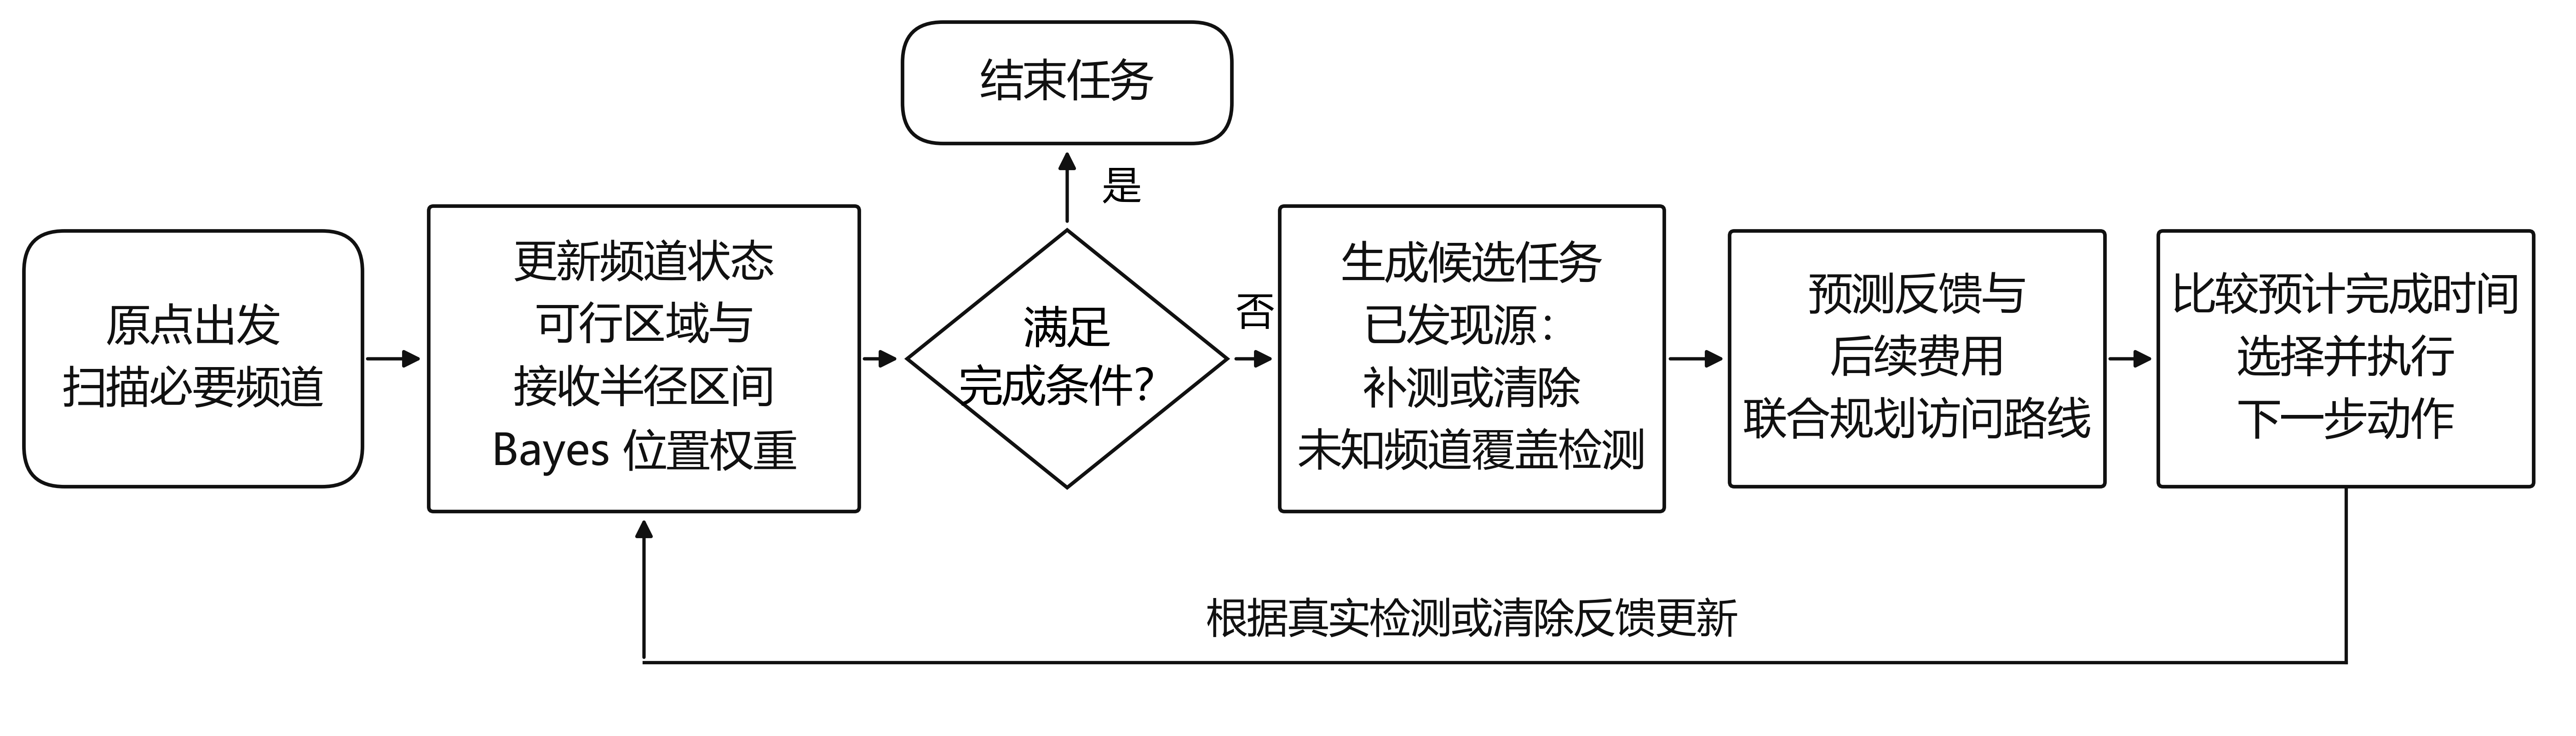
\includegraphics[width=\linewidth]{data/q3_bayes_flowchart_bw_horizontal/q3_bayes_flowchart_bw_horizontal.png}
  \caption{Bayes 搜索定位与清除的整体流程}
  \label{fig:q3-flow}
\end{figure}

\subsubsection{算法实现细节与边界处理}

\textbf{评分与路线求解。}我们声明：式~\eqref{eq:q3-score} 是便于在线求解的剩余费用近似，
\textbf{不能}视作全局最优策略的精确价值函数。
当待访问的代表点与覆盖测站总数较少时，采用\textbf{动态规划}求解固定点的访问顺序，
规模较大时采用\textbf{局部调整算法}（2-opt等）。每轮仅执行选中的下一步动作，获得真实反馈后再更新路线。
% 后续补充：实际版本的候选动作、路线规模阈值及局部改进规则。

\textbf{清除尝试与失败处理。}记频道 $c$ 当前的完整可行区域为 $P_{c,t}$，
能够保证清除的条件为
\begin{equation}
  P_{c,t}\subseteq B(\boldsymbol q,20).
  \label{eq:q3-safe-clear}
\end{equation}
当这一条件尚未满足，但后验给出的清除成功概率较高时，仍可将尝试清除与继续检测作费用比较，
并将失败后的补测成本计入。\textbf{只有收到成功反馈才将该源标记为已清除}；
失败反馈用于排除本次清除范围内的位置，再继续定位。
若收到“距离过近”反馈，由于源距检测点不超过 $5\,\mathrm m$，可\textbf{直接转入清除}。

\textbf{频道排除与停止条件。}对于未发现信号的频道，利用接收半径至少为
$1000\,\mathrm m$ 的条件安排覆盖检测。只有该频道全部剩余候选位置都被已执行的
无信号检测排除，才能判定其不存在。因此，停止条件为：已发现源均已成功清除，
且其余频道均已排除；或者已成功清除 $16$ 个不同频道的源，由题设数量上限可以确认任务完成。
覆盖状态仅由真实反馈更新，规划中的预期扫描不能提前计作已完成任务。

\subsubsection{全知者参照与结果验证}

为判断任务耗时的主要来源，除统计演练结果外，引入已知全部源位置的全知者参照。
该参照省去发现源、测向和确认无遗漏的过程，仅计算从原点出发访问全部源的最短开放路径。
其作用是给出物理移动成本的量级，帮助解释实际算法的费用，而不是替代在线策略。

记全知条件下的源坐标为 $\boldsymbol g_1,\ldots,\boldsymbol g_N$。
令 $D(S,j)$ 表示从原点出发、访问集合 $S$ 中的源并在 $j$ 处结束的最短路程，
则有
\begin{equation}
  \begin{aligned}
    D(\{j\},j)&=\|\boldsymbol g_j\|,\\
    D(S,j)&=\min_{i\in S\setminus\{j\}}
       \left[D(S\setminus\{j\},i)+\|\boldsymbol g_i-\boldsymbol g_j\|\right],\\
    L_0&=\min_j D(\{1,\ldots,N\},j).
  \end{aligned}
  \label{eq:q3-oracle}
\end{equation}
动态规划的时间复杂度为 $O(N^2 2^N)$。本题 $N\leq16$，可对每张参照地图精确求解，
相应纯移动时间为 $L_0/5$。

实际清除允许在距源 $20\,\mathrm m$ 内完成，因此逐点访问的 $L_0$ 并非原任务的严格下界。
若 $L_{20}$ 表示允许在各清除圆盘内自由选点的最短路程，则
\begin{equation}
  \max\{0,L_0-20(2N-1)\}\leq L_{20}\leq L_0.
  \label{eq:q3-oracle-bound}
\end{equation}
右侧由直接访问源坐标得到；左侧将圆盘内访问点移至对应源坐标，
首段路程至多增加 $20\,\mathrm m$，其余 $N-1$ 段各至多增加 $40\,\mathrm m$。
由此可在保留清除范围差异的前提下比较移动成本。

参照实验采用给定源数下的圆域面积均匀位置模型，源数分别使用
$10$ 至 $16$ 的等概率分布和演练记录的经验频率。
位置模型作为模拟假设单独说明，不能仅由源数统计推出。
汇总比较统一使用“总时间除以总源数”的口径，并将实际算法的移动、检测、切频和清除费用分别列出。
若全知者地图与演练地图未配对，两者的比值只能解释为\textbf{模型条件下的量级比较}，
不能写成逐图近似比或最优性证明。
% 已有全知者附件报告：100000张随机地图；经验源数加权135.6455 s/源（纯移动）。
% 附件的Bayes官方50轮为669/669、214.8761 s/源；待核对具体版本与原始日志后填入正文。

\begin{figure}[htbp]
  \centering
  \fbox{\parbox[c][2.6cm][c]{0.92\linewidth}{\centering\small
    验证图预留\\[0.5em]
    左：代表案例的移动路线、检测点及清除点\\
    右：实际策略的费用分解与全知者移动参照}}
  \caption{任务执行过程与时间费用对比（预留）}
  \label{fig:q3-validation}
\end{figure}

演练结果首先检查源的清除比例，再报告平均定位清除时间与实际运行时间。
对多局实验，同时保留逐局结果和汇总结果，避免将各局时间/源数的等权平均
与总时间/总源数混用。数值核验包括路线距离与动作费用对账、完成条件检查，
以及位置网格和角度分档加密后的策略稳定性。
三次正式测试按题设格式列于表~\ref{tab:q3-official}，结果及案例编码待实际测试后填写，
对应日志以模拟器导出的原文件名纳入支撑材料。

\begin{table}[htbp]
  \centering
  \caption{问题三正式测试结果（待填）}
  \label{tab:q3-official}
  \small
  \renewcommand{\arraystretch}{1.25}
  \begin{tabularx}{0.96\linewidth}{Xccc}
    \toprule
    测试案例编码 & 清除干扰源个数 & \shortstack{平均定位清除\\时间/(s/源)} & 程序运行时间/s \\
    \midrule
    测试1：待填 & --- & --- & --- \\
    测试2：待填 & --- & --- & --- \\
    测试3：待填 & --- & --- & --- \\
    \bottomrule
  \end{tabularx}
\end{table}

\subsection{问题四模型建立与求解}
\label{sec:q4}
% 本节采用21点覆盖布局；算法及实验版本以支撑材料中的记录为准。

问题三中的干扰源向各个方向发射信号，机器狗收不到信号时，可以根据接收半径排除附近的一部分区域。
本问中，定向源只向前方半个平面辐射。即使机器狗已经接近干扰源，也可能因位于其背面而收不到信号。
因此，本问首先需要解决的是：\textbf{怎样利用不同位置的检测，判断一个区域内是否仍可能存在干扰源。}

在此基础上，还需选择有利于定位的测点，并安排搜索与清除的先后顺序。
我们沿用问题三的时间评价，将多点检测的几何判断与 Bayes 位置更新结合起来。
下面先说明定向性如何改变检测结果，再建立覆盖搜索与定位清除的方法。

\subsubsection{定向源的接收条件}

以频道 $c$ 区分干扰源，记其候选位置为 $\boldsymbol z$，接收半径为 $R_c$。
对于定向源，用单位向量 $\boldsymbol u_c$ 表示发射方向。
测点能否收到信号，取决于两个条件：一是距离不超过接收半径，二是位于发射方向的前方。
题设将发射方向两侧各 $90^\circ$ 的边界也计入辐射范围，因此接收条件为
\begin{equation}
  \|\boldsymbol p-\boldsymbol z\|\leq R_c,\qquad
  \boldsymbol u_c^{\mathsf T}(\boldsymbol p-\boldsymbol z)\geq0.
  \label{eq:q4-reception}
\end{equation}
其中，$\boldsymbol p$ 为检测点，$\boldsymbol p-\boldsymbol z$ 是从源指向检测点的向量。
第二个不等式判断该向量在发射方向上的投影：投影为正时，测点在源的前方；
为零时在辐射边界上；为负时在背面。全向源没有朝向限制，只需满足第一个不等式。

例如，假定源向正东方向发射，则源东侧及正南、正北边界上的测点，只要距离足够近，就能收到信号；
源西侧的测点则收不到信号。因此，\textbf{无信号既可能表示距离过远，也可能表示测点位于背面}。
一次无信号检测不能像问题三中那样，直接排除测点周围半径 $1000\,\mathrm m$ 的圆域。

收到信号后，仍按题设的距离条件区分两种反馈：距离大于 $5\,\mathrm m$ 时返回示向度，
不超过 $5\,\mathrm m$ 时返回“距离过近”。正常示向用于构造第一问中的楔形区域，
再与已有的候选位置区域求交。

实际示向度保留两位小数。为避免舍入使真实位置落到计算区域之外，在 $1^\circ$ 测角误差之外，
再预留 $0.005^\circ$，即采用 $1.005^\circ$ 的楔形半角。
同一频道在同一位置的误差固定，因此原地重复检测不能提供新的独立测向信息。

\subsubsection{多个无信号测点的联合排除}

单个测点可能处于源的背面，但若测点从不同方向围住候选位置，它们便不可能同时位于背面。
利用这一几何关系，可以将多次无信号检测结合起来，排除一部分源位置。

设同一频道在三个不共线测点 $\boldsymbol p_i,\boldsymbol p_j,\boldsymbol p_k$ 均未收到信号。
考虑这些测点围成的三角形，并从中保留到三个测点的距离都不超过 $1000\,\mathrm m$ 的部分，记为
\begin{equation}
  E_{ijk}=\operatorname{conv}\{\boldsymbol p_i,\boldsymbol p_j,\boldsymbol p_k\}
  \cap B(\boldsymbol p_i,1000)\cap B(\boldsymbol p_j,1000)\cap B(\boldsymbol p_k,1000).
  \label{eq:q4-exclusion}
\end{equation}
式中，$\operatorname{conv}$ 表示三点的凸包，即包含边界的三角形；
$B(\boldsymbol p,1000)$ 表示以 $\boldsymbol p$ 为圆心、半径为 $1000\,\mathrm m$ 的闭圆盘。
三角形约束保证测点围住候选位置，三个圆盘约束则保证距离不妨碍信号接收。

下面说明为什么区域 $E_{ijk}$ 可以被排除。
假设该频道的源位于其中一点 $\boldsymbol z$。由于接收半径至少为 $1000\,\mathrm m$，
三个测点都处于其接收距离以内。若三点仍全部无信号，就只能说明它们都在源的背面。

但 $\boldsymbol z$ 位于三角形内，可写成三个顶点的加权平均：
\[
  \boldsymbol z=\lambda_i\boldsymbol p_i+\lambda_j\boldsymbol p_j+\lambda_k\boldsymbol p_k,
  \qquad
  \lambda_i,\lambda_j,\lambda_k\geq0,\quad \lambda_i+\lambda_j+\lambda_k=1.
\]
将等式两侧减去 $\boldsymbol z$，再沿发射方向取投影，得到
\[
  \sum_{a\in\{i,j,k\}}\lambda_a
  \boldsymbol u_c^{\mathsf T}(\boldsymbol p_a-\boldsymbol z)=0.
\]
若三点都在背面，各项投影均为负，其加权平均也应为负，与上式矛盾。
所以至少有一个测点应该收到信号。由此可知，\textbf{三个无信号记录足以排除 $E_{ijk}$ 内存在该频道的源}。
对于全向源，距离条件本身就已保证能够接收，故同样可以排除这一区域。

每增加一个无信号测点，就将它与已有测点组成新的三点组合，并从候选位置区域中扣除相应的 $E_{ijk}$。
这些记录必须来自同一频道。例如，对频道1的无信号检测，只能用于排除频道1的候选位置，
不能作为频道2已完成检测的依据。

\subsubsection{覆盖测点的布置}

前述判据解决了局部区域的排除问题。为了搜索整个目标圆域，还需布置足够的测点，
使域内每个位置都能被一组距离足够近的测点围住。
若某个频道在这些位置依次检测后始终没有信号，就能确认目标域内不存在该频道的源。

我们采用原点、内圈8点和外圈12点组成的21点布局。
内圈距原点约 $998\,\mathrm m$，外圈距原点约 $1866\,\mathrm m$，各点的整数坐标列于支撑材料。
外圈略超出源的分布圆域，是为了从外侧检测靠近边界且朝外发射的源。
题设限制的是源的分布范围，允许机器狗到圆域外检测。

测点布置后，还需要验证测点之间是否留下了无法搜索的空隙。
为此，将目标圆域所在的方框逐级四等分，对与目标域相交的每个小方格作检查。
如果小方格的四个角点均位于一组附近测点的凸包内，并且到这些测点的距离均小于
$999\,\mathrm m$，则保留该方格；否则继续细分。

这里检查四角就足够，是因为方格内任一点都可表示为四角的加权平均。
四角在凸包内，整个方格也在凸包内；四角在某个接收圆盘内，整个方格也在该圆盘内。
因此，方格内任何位置都有一组距离足够近、且将它围住的测点。
上一节的投影证明对三个以上的测点同样成立，所以其中至少一点能收到信号。

该布局共通过 $3832$ 个方格的检查，各方格所用测点到其角点的最大距离约为
$998.79\,\mathrm m$，目标圆域边界也包含在检查范围内。
此外，将布局中全部三点组合的排除区域取并集，复核其覆盖整个目标圆域。
这两项检查共同验证了所用布局的覆盖能力。

机器狗不必在每场任务中走完全部21个测点。
当某些频道已被发现、清除或排除，剩余测点承担的检测任务也随之减少。
删除或移动测点之前，重新检查已有检测位置与剩余测点能否完成各频道的搜索。
只有检查通过才调整路线；预计将要进行的检测，不能提前计作已经得到的无信号记录。

\subsubsection{考虑发射方向的 Bayes 位置更新}

几何约束保留了所有尚未排除的位置，但不同位置解释已有观测的可能性并不相同。
与问题三一样，我们利用 Bayes 更新计算位置概率，作为后续选点的依据。
本问增加的未知量是源的类型与发射方向，需要将它们和接收半径一起考虑。

首先沿用前文的位置假设：源在目标圆域内按面积均匀分布。
对于未知的接收半径，仍假设其在 $[1000,1500]\,\mathrm m$ 内均匀分布，
即等长的半径区间具有相同的初始概率。

对于新增的类型与方向信息，全向、定向两类源的初始概率各取 $1/2$。
若为定向源，则假设其发射方向在整周内均匀分布，等宽的朝向角区间具有相同的初始概率。
这里没有假定一场任务中恰有一半源为定向源，只是在尚未观测时对两种类型赋予相同的可能性。

上述未知量在初始假设中相互独立。这些分布描述的是我们尚未掌握的信息；
同一源实际具有的类型、半径和朝向，在整场任务中均保持不变。

\textbf{先判断一个候选位置能否解释全部记录。}
以某个候选位置为原点，假设三个检测点的相对坐标依次为
$(1200,0)$、$(-800,0)$ 和 $(1300,0)$，单位为米，反馈依次为有信号、无信号和无信号。
下面依次分析这三条记录对该候选位置的要求。

第一个测点位于候选位置东侧，距离为 $1200\,\mathrm m$。
能够收到信号，说明接收半径至少为 $1200\,\mathrm m$；
如果该源为定向源，其发射范围还必须包含东方。

第二个测点位于西侧，距离只有 $800\,\mathrm m$，小于题设的最小接收半径。
它没有收到信号，因此在这个候选位置上，全向源的解释不成立；
若为定向源，则西侧必须处于发射背面。
结合第一条记录，允许的发射朝向位于朝东的半周内，不含正南、正北两个边界方向。

第三个测点与第一个测点都在东侧，因此也应处于信号辐射范围内。
它在 $1300\,\mathrm m$ 处没有收到信号，只能由接收距离不足来解释。
合并三条记录后，允许的接收半径为
\[
  1200\leq R_c<1300\qquad(\mathrm m).
\]
这一例子说明，同一条无信号记录是否限制半径，取决于测点与源的相对方向。
只有将不同位置的记录放在一起，才能得到正确的参数范围。

\textbf{再计算这些记录在候选位置上出现的概率。}
仍看上面的例子，并先只考虑是否收到信号。
初始假设中，源为定向源的概率是 $1/2$；
在定向源的全部朝向中，朝东的半周占 $180^\circ/360^\circ=1/2$；
允许的半径区间长 $100\,\mathrm m$，占初始半径范围的 $100/500=1/5$。
这三项在初始假设中相互独立，因而三次接收结果同时出现的概率为
\[
  \frac12\times\frac12\times\frac15=0.05.
\]
也就是说，假定源就在这个候选位置，初始假设中有 $5\%$ 的类型、朝向和半径组合
能够解释这三次接收记录。这个概率随后用于比较不同候选位置。

一般情况下，允许的朝向不一定恰好是半周。
固定候选位置，让假定的发射方向转过一周，测点只有越过辐射范围的两条边界时，
才会在前方与背面之间转换。以发生转换的朝向为分界，将一周划分成若干段，
则每一段内部各测点的前后关系保持不变。

对于其中一段朝向，若有信号的测点落在背面，这一段就无法解释观测，应予以排除。
其余情况下，收到信号的最远测点决定接收半径至少应有多大；
位于前方却没有信号的测点中，最近的一个决定接收半径必须小于多大。
将这两个要求与题设的 $[1000,1500]\,\mathrm m$ 范围合并，就得到这一段朝向允许的半径区间。
若没有半径同时满足这些要求，该段朝向也不成立。

随后，按上例将类型概率、该段角度占比和半径区间占比相乘。
各段朝向互不重叠，故可以将结果相加；全向情形若也能解释记录，则再加入全向情形对应的概率。

正常示向还提供了角度信息。假定一个候选位置后，可以算出从各测点指向它的真实方位。
实测读数保留两位小数，因而对应一个宽 $0.01^\circ$ 的舍入区间。
将这个区间减去真实方位，就得到测角误差必须落入的范围。
再与题设的 $[-1^\circ,1^\circ]$ 取交集，便得到能够产生该读数的误差范围。

根据第二问的均匀误差假设，将上述交集的角度宽度除以 $2^\circ$，即为出现这一读数的概率。
不同检测位置的误差按前文假设独立处理，因此各次读数的概率相乘，再乘以前述接收概率，
便得到该候选位置产生已有检测记录的概率。同一位置的重复记录只计一次。

\begin{samepage}
\textbf{最后把各候选位置的计算结果转为位置概率。}
沿用第二问的网格计算方法，将当前可行区域划分为小区域。
在每个小区域内取一个点，代表该区域中可能的源位置。
用 $\ell$ 表示区域编号，$A_\ell$ 表示其面积，
$q_\ell$ 表示假定源位于该代表位置时，产生已有检测记录的概率。
根据面积均匀先验，第 $\ell$ 个区域在观测后的概率近似为
\begin{equation}
  w_\ell=\frac{A_\ell q_\ell}{\sum_j A_jq_j}.
  \label{eq:q4-position-weight}
\end{equation}
分子将该区域原有的面积权重与观测出现的概率相乘；
分母的下标 $j$ 遍历全部小区域，对它们的同类结果求和，使更新后的概率之和为 $1$。
因此，面积相同的两个区域中，能够以更大概率产生已有观测的区域，会获得更大的位置权重。
式~\eqref{eq:q4-position-weight} 用代表位置近似整个小区域，数值精度取决于区域划分的细致程度。
\par
\end{samepage}

计算时，先用面积最小的外接矩形包住可行区域，矩形允许随区域的延伸方向旋转。
在矩形内划分 $16\times16$ 网格，再用可行区域裁剪各网格，以保留下来的面积作为 $A_\ell$。
若全部网格的计算权重均为零，则加密到 $32\times32$。
即使加密后仍无法计算，也不能据此判定源不存在，而应保留可行区域并采用后文的后备搜索。

\subsubsection{搜索、定位与清除的安排}

获得位置概率后，需要判断下一次到哪里检测，以及是否应当先处理其他源。
这一安排仍以完成任务的时间为依据，总时间按式~\eqref{eq:q3-time} 计算。
其中，机器狗移动速度为 $5\,\mathrm{m/s}$，移动 $1000\,\mathrm m$ 就需要 $200\,\mathrm s$，
因此，为改善交会角而增加的路程必须计入选点费用。

对于一个已发现的源，先构造几类候选测点：沿示向接近源的点、向侧面偏移的点，
以及附近其他源或覆盖测点的位置。
沿示向接近主要减少后续移动；侧向偏移可以改善两次测向的交会角；
附近任务位置则可能在完成本次检测后，减少前往下一任务的路程。

与第二问一样，选点时尚不知道将得到哪种反馈。
因此，对每个候选点分别预测正常示向、距离过近和无信号的概率，
估计各类反馈出现后还要花多少时间完成该源的定位与清除，再按反馈概率加权平均。
将这一平均费用与前往测点的移动、切频及检测时间相加，得到该候选点的局部费用。
这样，一个交会角较好的点，如果很可能位于源的背面，也未必优于较近的测点。

预测时将示向角分档，先用 $10^\circ$ 的档宽比较候选点，再用 $2^\circ$ 的档宽细算入选点。
这些角度档用于计算尚未获得的反馈，不改变实际测向后的误差范围。
局部费用中还估计了尝试清除失败后需要补测和移动的时间，避免把失败后的工作漏掉。

接着，将已发现源的代表位置和剩余覆盖测点共同纳入路线规划。
沿用式~\eqref{eq:q3-score}，把当前任务的局部费用与其他任务的访问费用合并比较，
确定下一步动作。每次取得实际反馈后，重新更新候选位置和路线。
路线只要求访问剩余任务，不要求最后返回原点。

\textbf{已有停留位置可以承担其他检测任务。}
例如，机器狗清除一个源后，若当前位置能够替代附近的某个覆盖测点，
并且替代后仍满足各频道的覆盖要求，就在这里检测相应频道。
不同频道仍要逐一切换、逐一检测，节约的是专门前往另一个位置的移动时间。

路线节点不超过16个时，用动态规划求解这些固定位置的访问顺序；
节点较多时，先构造最近邻路线，再交换部分路段以缩短距离。
由于后续观测会改变源的代表位置，且尚未发现源的定位行程仍未知，
当前路线及费用只作为下一步选择的依据，不能解释为整个任务的最优解。

清除判断沿用问题一的最小覆盖圆方法。
如果完整可行区域能被半径 $20\,\mathrm m$ 的圆覆盖，机器狗到达圆心后，
到所有可能源位置的距离都不超过清除半径，因而可以保证清除。
收到“距离过近”时，则可直接在该检测点清除。

尚不满足上述条件时，也可将尝试清除与继续检测作时间比较。
只有收到成功反馈才将该源记为已清除；失败反馈说明源不在本次清除点的
$20\,\mathrm m$ 范围内，可扣除这一部分位置后继续定位。
清除是否成功只与距离有关，不受发射朝向影响。

为避免多次补测后仍不能完成定位，保留按方格逐个清除的后备方法。
沿首次示向方向，用边长 $20\,\mathrm m$ 的方格覆盖剩余可行区域，并依次访问有关方格的中心。
方格内任一点到中心的距离至多为 $10\sqrt2\,\mathrm m$，小于清除半径，
因此有限个方格中心即可覆盖这个有界区域。
对于尚未发现的频道，则保留间距 $700\,\mathrm m$ 的方格测点补充搜索；
每个方格的对角线小于 $1000\,\mathrm m$，可利用三点排除判据检查是否存在遗漏。

数值计算也应保持这一完整性。
用多边形近似曲线边界时，可能存在源的区域从外侧包住，能够排除的圆盘从内侧近似，
使近似误差只会减少已排除区域，不会误删真实源位置。
只要还有未排除区域，就继续保留对应搜索任务。

当全部20个频道均已清除或被实际检测排除，任务才算完成。
另一种情况是已成功清除16个不同频道的源，由题设数量上限可直接结束。
如果只是发现了16个源，仍需完成它们的清除。
上述后备方法保留了有限完成途径，能否在规定时间内做完，还需由实验检验。

\subsubsection{实验结果与分析}

为考察测点布置对任务时间的影响，在相同地图上比较21点布局与22点布局。
22点布局由原点、内圈7点和外圈14点组成，两种布局使用相同的定位、选点、路线规划和停止规则。
因此，同一张地图上的用时差异，可以用于评价布局变化在完整任务中的作用。

实验分为两组。第一组包含16张随机地图，源数取10至16，接收半径在题设范围内变化，
每张地图同时包含全向源和定向源。
第二组包含14张压力地图，用于考察随机地图中不容易充分出现的情形。
其中包括源靠近边界、朝外发射、沿边界切向发射、多个源聚集，以及机器狗位于源附近或背面的情况；
同时采用接收半径的边界值、极端测角误差或空间相关误差。

每对实验共用源位置、频道、接收半径和发射方向，同一地点的测角误差也保持一致。
两种布局各运行30场，均完成全部清除，并满足停止条件，未出现超时或运行失败。
总虚拟时间计入移动、切频、检测及清除，统计结果见表~\ref{tab:q4-paired}。
% 实验批次：20260913-013804-paper-q4-recheck，完整参数、动作及复核结果见同名支撑材料。
% 随机种子800--815；压力种子9100--9113。数据沿用本批60场完整复跑，不混用历史结果。

\begin{table}[htbp]
  \centering
  \caption{两种覆盖布局的同图实验结果}
  \label{tab:q4-paired}
  \small
  \begin{tabular}{lrrrr}
    \toprule
    地图组 & 配对数 & \shortstack{22点布局\\平均总时间/s}
      & \shortstack{21点布局\\平均总时间/s} & 时间变化 \\
    \midrule
    随机地图 & 16 & 5794.55 & 5670.72 & $-2.14\%$ \\
    压力地图 & 14 & 5932.66 & 5721.44 & $-3.56\%$ \\
    合计 & 30 & 5859.00 & 5694.39 & $-2.81\%$ \\
    \bottomrule
  \end{tabular}
  \par\smallskip
  \parbox{0.94\linewidth}{\footnotesize 注：时间变化为21点布局相对22点布局的平均总时间变化；
  合计按30场等权计算。两种布局在各组中均全部完成。}
\end{table}
\FloatBarrier

在30对实验中，21点布局有19对用时更少，平均每场节约 $164.61\,\mathrm s$。
表~\ref{tab:q4-costs} 进一步列出路程与动作次数。
平均移动路程由 $21.019\,\mathrm{km}$ 降至 $20.384\,\mathrm{km}$，
对应节约移动时间约 $126.85\,\mathrm s$。可见，总用时的下降主要来自路程减少，
检测、切频及失败清除次数的减少也带来了一部分收益。

\begin{table}[htbp]
  \centering
  \caption{两种布局的平均路程与动作指标}
  \label{tab:q4-costs}
  \begin{tabular}{lrr}
    \toprule
    指标（每场均值） & 22点布局 & 21点布局 \\
    \midrule
    移动路程/km & 21.019 & 20.384 \\
    检测次数 & 267.47 & 261.00 \\
    失败清除次数 & 2.43 & 2.00 \\
    平均定位清除时间/(s/源) & 479.35 & 467.72 \\
    实际计算时间/s & 6.06 & 5.34 \\
    \bottomrule
  \end{tabular}
  \par\smallskip
  \parbox{0.94\linewidth}{\footnotesize 注：平均定位清除时间先按每场总虚拟时间除以清除源数，
  再对30场取均值。实际计算时间为同一机器上的运行记录，不计入机器狗的虚拟耗时；
  实验环境与参数见支撑材料。}
\end{table}
\FloatBarrier

这里的路程包含了发现源后的定位与清除行程，不只是依次走完覆盖测点的距离。
如果只计算初始覆盖测点的访问路线，同一路线求解器给出的22点与21点布局路程分别为
$17.639\,\mathrm{km}$ 和 $17.909\,\mathrm{km}$，21点布局反而稍长。
但实际运行中，源被发现的时机和位置会影响后续安排，部分测点也可能不再需要访问。
因此，布局的效果应根据完整任务判断，不能仅由初始路线长度确定。

平均用时减少，也不表示每张地图都会改善。
在一张10个源聚集的压力地图中，全部源均为定向源，接收半径为 $1000\,\mathrm m$，并采用极端测角误差。
21点布局的总时间为 $6451.10\,\mathrm s$，高于22点布局的 $5665.03\,\mathrm s$，增加 $13.88\%$。
这一结果表明，该布局在部分情形下仍会增加搜索清除费用。

为进一步判断平均节约是否稳定，对16张随机地图的同图时间差作配对 $t$ 检验。
所得 $p$ 值为 $0.079$，大于 $0.05$，即在 $5\%$ 显著性水平下，还不足以确认平均时间存在差异。
因此，本批实验说明21点布局在这些地图上取得了小幅平均改进，
但有限样本尚不能证明它在其他地图上也稳定优于22点布局。
14张人为构造的压力地图主要用于检查特殊情形，不用于推断正式测试的平均成绩。

\begin{samepage}
以上为本地模拟结果。三次正式测试按题设格式列于表~\ref{tab:q4-official}，
待取得实际结果后填写，对应导出日志纳入支撑材料。
\par
\end{samepage}
\begin{table}[htbp]
  \centering
  \caption{问题四正式测试结果（待填）}
  \label{tab:q4-official}
  \small
  \renewcommand{\arraystretch}{1.25}
  \begin{tabularx}{0.96\linewidth}{Xccc}
    \toprule
    测试案例编码 & 清除干扰源个数 & \shortstack{平均定位清除\\时间/(s/源)} & 程序运行时间/s \\
    \midrule
    测试1：待填 & --- & --- & --- \\
    测试2：待填 & --- & --- & --- \\
    测试3：待填 & --- & --- & --- \\
    \bottomrule
  \end{tabularx}
\end{table}
\FloatBarrier

\section{模型检验与合理性分析}

\begin{figure}[htbp]
  \centering
  \caption{模型计算结果}
  \label{fig:result}
\end{figure}

如图~\ref{fig:result} 所示，模型结果呈现出……

\section{模型评价与展望}

\subsection{模型评价}
可以分优点和缺点

\begin{itemize}
  \item 模型结构清晰，具有较强的可解释性；
  \item 计算复杂度较低；
  \item 可以推广到其他类似问题。
\end{itemize}

\subsection{未来展望}
···


\begin{thebibliography}{99}

\bibitem{boyd2004convex}
Boyd S, Vandenberghe L.
Convex Optimization[M].
Cambridge: Cambridge University Press, 2004: 34, 36.
% 第2.2.4节：有界多面体的顶点表示；第2.3.1节：交集保凸性。
% 作者公开全文：https://web.stanford.edu/~boyd/cvxbook/bv_cvxbook.pdf

\bibitem{ref1}
张三, 李四.
数学建模方法与应用[M].
北京: 某出版社, 2025.

\bibitem{ref2}
Author A, Author B.
Title of the article[J].
Journal Name, 2024, 10(2): 1--10.

\end{thebibliography}

\end{document}
